%% =========================================================================
%% Master's Dissertation — PPGCC, CIn-UFPE — ENGLISH VERSION
%% Template: risethesis (CIn class), option [en]
%% Adapted (not literally translated) from dissertacao/, which remains the
%% deposit reference; this version targets international dissemination.
%% Compile: tectonic main.tex (or pdflatex -> bibtex -> pdflatex x2)
%% =========================================================================
\documentclass[en,oneside,onehalfspacing,msc]{risethesis}

\usepackage{babel}% the class passes [brazil,english]; english is primary
\usepackage{color}
\usepackage[table]{xcolor}
\usepackage{microtype}
\usepackage{multirow}
\usepackage{rotating}
\usepackage{booktabs}
\usepackage{caption}
\usepackage{float}
\usepackage{subcaption}
\usepackage{amsmath,amssymb}
\usepackage{textcomp}
% Escape valve for paragraphs with long tokens (artifact paths in \texttt):
\emergencystretch=1.5em
% tikz is not in the preamble: diagrams are pre-compiled into
% images/tikz-*-en.pdf (editable sources in tikz-src/).
\setcounter{secnumdepth}{3}
\setcounter{tocdepth}{2}

%% ---- Title format following the CIn dissertation standard ----
\titleformat{\chapter}[hang]
  {\normalsize\bfseries}{\thechapter}{1em}{\MakeUppercase}
\titleformat{name=\chapter,numberless}[hang]
  {\normalsize\bfseries\filcenter}{}{0pt}{\MakeUppercase}
\titlespacing*{\chapter}{0pt}{0pt}{24pt}
\titleformat{\section}
  {\normalsize}{\thesection}{1em}{\MakeUppercase}
\titleformat{\subsection}
  {\normalsize\bfseries}{\thesubsection}{1em}{}
\titleformat{\subsubsection}
  {\normalsize\itshape}{\thesubsubsection}{1em}{}
\captionsetup{font=small,labelfont=small,skip=6pt}

\newcommand{\us}{\textmu s}

\address{RECIFE}
\universitypt{Universidade Federal de Pernambuco}
\universityen{Federal University of Pernambuco}
\institutept{Centro de Informática}
\instituteen{Center for Informatics}
\programpt{Pós-graduação em Ciência da Computação}
\programen{Graduate Program in Computer Science}
\majorfieldpt{Ciência da Computação}
\majorfielden{Computer Science}

% PROVISIONAL title — mirrors the Portuguese title; the word "Validated"
% (like "Validado" in the PT version) is pending the author's decision.
\title{Models for Tabular Data in the Era of Foundation Models:
a Multi-Criteria Benchmark, an Evaluated Decision Framework, and
Distributional Distillation}

\date{2026}
\author{João Gabriel de Araújo Vasconcelos}
\adviser{Germano Crispim Vasconcelos}

% \includeonly{chapters/cap7-destilacao}

\usepackage{array}
% Cabeçalho corrente (lote 25/11): título curto já na página de abertura
% da seção — \hdrshort{...} antes de \section{...} declara o mark curto
% que o \sectionmark automático do \section usará uma única vez.
\makeatletter
\gdef\hdr@short{}
\newcommand{\hdrshort}[1]{\gdef\hdr@short{#1}}
\renewcommand{\sectionmark}[1]{%
  \ifx\hdr@short\@empty
    \markright{\MakeUppercase{\thesection.\ #1}}%
  \else
    \markright{\MakeUppercase{\thesection.\ \hdr@short}}\gdef\hdr@short{}%
  \fi}
\makeatother
% Correção (lote 25/11): o estilo plain da classe usa \fancyhead sem
% seletor e desenha o número da página 3x sobreposto (L, C e R, todos
% com \hfill) nas aberturas de capítulo; aqui, uma única vez, à direita.
\fancypagestyle{plain}{%
  \fancyhead{}\fancyfoot{}%
  \fancyhead[R]{\rule{0cm}{4mm}\thepage}%
  \renewcommand{\headrulewidth}{0pt}}
% URLs: não quebrar logo após o ':' (evita "https:" órfão na bibliografia)
\expandafter\def\expandafter\UrlNoBreaks\expandafter{\UrlNoBreaks\do\:}
% terceira passada de quebra: elimina os estouros marginais (~1 mm)
% de \texttt longos sem afrouxamento visivel
\setlength{\emergencystretch}{1.5em}
% paginas so de float: alinhar no topo, nao centrar no vazio
\makeatletter
\setlength{\@fptop}{5pt}
\setlength{\@fpbot}{0pt plus 1fil}
\makeatother
\usepackage{pdflscape}
% Diagramação (lote 25/11): floats podem dividir página com texto
\renewcommand{\topfraction}{0.9}
\renewcommand{\bottomfraction}{0.6}
\renewcommand{\textfraction}{0.07}
\renewcommand{\floatpagefraction}{0.66}
\setcounter{topnumber}{3}\setcounter{totalnumber}{5}

\begin{document}

\frontpage
\presentationpage

\begin{fichacatalografica}
% Blank page: the catalog card is produced by the library at deposit time.
\end{fichacatalografica}

% Approval sheet: PLACEHOLDER page reserved; the sheet itself is
% produced by the graduate office after the defense.
\newpage\thispagestyle{empty}\vspace*{\fill}
\begin{center}\itshape [Approval sheet --- page reserved; issued by
the graduate office after the defense]\end{center}
\vspace*{\fill}\clearpage

\acknowledgements
%% ============================================================================
%% Acknowledgements (B16, 2026-11-26): personalized per the author's
%% direct order, adapted (not copied) from his 2023 undergraduate
%% thesis. Confirmed by the author (26/11): the four family names;
%% no funding agency to acknowledge. Still flagged for his review:
%% the CloudWalk sentence on serving cost.
%% ============================================================================
My first thanks go to my family. To my parents, Wilmar and Maria do
Socorro, who trusted my choices before I could justify them and who
stand behind everything I manage to do. To my brother Rafael and my
sister Luana, who were my references long before I knew what a
reference was, and whose encouragement in the hard weeks counted for
as much as the celebration in the good ones.

To Professor Germano Crispim Vasconcelos, who has now advised me
twice. This dissertation picks up a question my undergraduate project
left open in 2023, namely whether the new neural models can compete with
gradient boosting on tabular data, and adds the question of what
that competition costs; it was his guidance, demanding rigor without
stifling curiosity, that turned those questions into a research
program. More than once a follow-up meeting changed the course of
this work for the better.

To the friends I made at CloudWalk, where I have worked throughout
this master's. You challenged me, encouraged me and influenced me,
and the problems we faced together kept alive the curiosity that
research depends on. It is no accident that this dissertation asks
what a model costs to serve, and not only how well it scores.

To my friends from Teresina, with whom I grew up and on whom distance
has had no effect, and to the friends who welcomed me in Recife and
became part of my life well beyond the university.

To the Centro de Inform\'atica at UFPE, its faculty and staff, for my
education from the undergraduate degree to this one, and to the
members of the examining committee, for the time and care given to
reading this work.

To everyone who questioned these results along the way: your
objections are answered in the text, which is better because of them.

To all who took part in this journey, directly or indirectly, my
sincere thanks.


\abstract
\enlargethispage{2\baselineskip}%
% Abstract (NBR 6028: one paragraph, no formulas).
For a decade, model selection for tabular data relied on the maxim that
gradient boosting always wins. Tabular foundation models, pre-trained
networks that predict without task-specific training, have cast doubt on it.
However, most available evidence comes from the proponents themselves, under
differing protocols. This dissertation produces evidence under a single
protocol and turns it into a selection procedure, along three lines. First,
a multi-criteria benchmark evaluates 14 models from three families
(gradient boosting, deep learning, and foundation models) on 18 OpenML
datasets, with a hold-out untouched by selection, frequentist and
Bayesian inference, and measured training, tuning, and latency costs.
Second, a decision framework is assessed: its learned component under
leave-one-dataset-out validation, its fixed policies descriptively. Third, the distillation of the TabPFN teacher's quantile curves into
gradient-boosting students is studied on 20 regression datasets, under registered
hypotheses. Among the 11 core models (prior to the 2026 extension), the top
of the accuracy ranking, measured in binary classification, is a tie. Other
tasks are read descriptively. Under a ROPE of one AUC percentage point,
3 of the other 10 models are practically equivalent to the leader, TabPFN, which is itself a foundation model,
by the strict Bayesian criterion, and 8 by the lenient one. In the 2026 generation, the untuned TabFM has the best average rank in all three tasks (in multiclass, over the two
datasets where it operates) and is the best model on 13 of 18 datasets
(operating on 17). The lead is consistent across datasets, but the
underpowered tests do not confirm it as a statistical separation, and this lead costs
about five orders of magnitude more latency on the reference dataset
(\texttt{adult}). Kolmogorov--Arnold networks finish in the bottom third on
all three tasks. For the decision, a router learned from meta-features is
less accurate than the trivial rule (0.11 vs.\ 0.44). The fixed
``foundation model first'' policy (an intra-family oracle) has zero median
regret on the primary metric, but stops being the recommendation
once 10 to 20 percent of the decision weight shifts from accuracy to
latency, by median regret, under rank normalization. In distillation, the
student trained on the teacher's means beats the control on only 4 of 20
datasets. The student trained on the quantile curves retains, at the
median, 12 to 19 percent of the distributional advantage, depending on how the arms are tuned, and retention is positive on 16 of 20 (sign test, p
approximately 0.019 after the sequential correction). It beats
default-configured classical distributional baselines on 17 of 20 (12 of 20
against the per-dataset best alternative). In the regime studied (up to 100
thousand samples, pinned versions, a single GPU), model choice should start
not from a universal winner but from the application's constraints:
latency, architectural limits, and auditable explanations. In this regime,
distillation recovers a modest median share of the foundation model's
predictive uncertainty, under preconditions measurable before training the student. The advantage gate was verified only in an oracle version, and
the rule was assessed only on the datasets it was derived from.

\vspace{0.4cm}
\noindent\textbf{Keywords:} tabular data; foundation models;
benchmarking; knowledge distillation; distributional regression.


\resumo
\enlargethispage{2\baselineskip}%
% Resumo (NBR 6028: um parágrafo, 150-500 palavras, sem fórmulas).
% Reescrito em 24/11/2026 (revisão pedagógica); todos os números conferidos
% nos capítulos e artefatos de origem antes da inclusão.
Por uma década, a escolha de modelos para dados tabulares apoiou-se na
máxima de que o \emph{gradient boosting} sempre vence. Os
\emph{foundation models} tabulares, redes pré-treinadas que predizem sem
treinamento na tarefa, puseram-na em dúvida. Contudo, a evidência vem sobretudo dos proponentes, sob protocolos
distintos. Esta dissertação produz evidência sob protocolo único e a
converte em procedimento de escolha, em três frentes. Primeiro, um
benchmark multicritério avalia 14 modelos de três famílias
(\emph{gradient boosting}, aprendizado profundo e \emph{foundation
models}) em 18 conjuntos do OpenML, com \emph{hold-out} intocado pela
seleção, inferência frequentista e bayesiana e custos de treino, ajuste e
latência medidos. Segundo, avalia-se um arcabouço de decisão: o componente
aprendido, sob validação \emph{leave-one-dataset-out}; as políticas fixas,
descritivamente. Terceiro, estuda-se a destilação das curvas de quantis do
professor TabPFN em alunos de \emph{gradient boosting}, em 20 conjuntos de
regressão, sob hipóteses registradas. Entre os 11 modelos do núcleo
(anteriores à extensão de 2026), o topo da acurácia na
classificação binária é um empate. As demais tarefas são lidas
descritivamente. Sob uma ROPE de um ponto percentual de AUC, 3 dos outros
10 modelos são praticamente equivalentes ao líder, o TabPFN, ele próprio um \emph{foundation model}, pelo critério bayesiano estrito, e 8 pelo brando, afirmação bem mais fraca. Na extensão de 2026, o TabFM, sem ajuste, tem o melhor
rank médio nas três tarefas (na multiclasse, sobre os dois conjuntos em que
opera) e é o melhor modelo em 13 dos 18 conjuntos (opera em 17). A
liderança é consistente entre conjuntos, mas os testes, de baixo poder, não
a confirmam como separação estatística, e ela custa cerca de cinco ordens de magnitude a mais em latência que o XGBoost no conjunto de referência (\texttt{adult}). As
redes Kolmogorov--Arnold ficam no último terço nas três tarefas. Na
decisão, um roteador aprendido por meta-características acerta menos que a
regra trivial (0,11 contra 0,44). A política fixa ``\emph{foundation
model} primeiro'' (um oráculo intrafamília) tem \emph{regret} mediano zero
na métrica primária, mas deixa de ser a recomendada quando 10 a 20
por cento do peso passa da acurácia à latência, pelo \emph{regret} mediano, na normalização por postos. Na destilação, o
aluno treinado nas médias do professor supera o controle em só 4 de 20. O aluno treinado nas curvas de quantis retém, na mediana, 12 a
19 por cento da vantagem distribucional, conforme o ajuste, com retenção positiva em 16 de 20 (teste de sinal, p aproximadamente 0,019
após a correção sequencial). Ele supera \emph{baselines} distribucionais
clássicos, em configuração \emph{default}, em 17 de 20 (12 de 20 contra a melhor alternativa por conjunto, via oráculo). No regime estudado (até 100 mil amostras,
versões fixadas, GPU única), a escolha deve partir não de um
vencedor universal, mas das restrições da aplicação: latência, limites
arquiteturais e explicações auditáveis. Nesse regime, a destilação
recupera, na mediana, uma parcela modesta da incerteza preditiva do
\emph{foundation model}, sob pré-condições mensuráveis antes do treino do
aluno. A regra de decisão foi avaliada apenas nos conjuntos de que foi derivada, e sua pré-condição, só em versão oráculo.

\vspace{0.4cm}
\noindent\textbf{Palavras-chave:} dados tabulares; foundation models;
benchmark; destilação de conhecimento; regressão distribucional.


%% PROVISIONAL translation of the author's AI-use declaration (an
%% author-owned zone in the PT version; wording subject to his decision).
\chapter*{Declaration of use of artificial-intelligence assistance}
\thispagestyle{empty}

This work used artificial-intelligence assistance (Claude, Anthropic)
as a support tool, under the author's continuous direction and review,
at the following stages: assisted drafting of the text from the
author's results, outlines, and decisions; assisted implementation of
experiment and analysis code; repeated, dated cross-checks between the
numbers in the text and the versioned artifacts that support them;
support in bibliographic searches and in the dated novelty checks
(with verification of primary sources); and organization of
presentation material. The research design, the hypotheses, the
methodological decisions, the selection of what to report ---
including the negative results --- and the final validation of every
claim are the author's.

Beyond writing support, on 2026-11-23 the text underwent an
\textbf{automated adversarial review}: an independent AI session,
without access to the writing context, instructed to act as an
examination committee --- recomputing numbers from the raw artifacts
(about 400 checks), re-running experiments, and confronting text,
code, and public record. The corrections arising from that review are
incorporated and recorded in the 2026-11-23 addendum to the
experimental design document and in the repository history; the
central checks were re-executed from the raw artifacts, on this same
assisted infrastructure, before being incorporated.

No experimental result was generated by a language model: every
number comes from artifacts produced by the versioned scripts of the
project's public repository, with fixed seeds and reproducible
execution. The development history is public in the repository, some
of the commits explicitly record the tool's co-authorship, and
corrections of record were made by dated rectification, never by
rewriting history.


\listoffigures
\listoftables
%% List of acronyms — manual (reference list in the CIn dissertation
%% standard; the text expands each acronym at first use).
%% EN adaptation: Portuguese glosses dropped; IC -> CI and QP -> RQ.
\chapter*{List of Acronyms}
\thispagestyle{empty}
\begin{description}\itemsep2pt
  \item[AI] Artificial Intelligence
  \item[AUC] Area Under the ROC Curve
  \item[AutoML] Automated Machine Learning
  \item[CD] Critical Difference (Nemenyi)
  \item[CDF] Cumulative Distribution Function
  \item[CI] Confidence Interval
  \item[CPU] Central Processing Unit
  \item[CQR] Conformalized Quantile Regression
  \item[CRPS] Continuous Ranked Probability Score
  \item[CTR23] the OpenML-CTR23 regression suite
  \item[CUDA] Compute Unified Device Architecture
  \item[DL] Deep Learning
  \item[FLOP] Floating-Point Operation
  \item[FM/TFM] (Tabular) Foundation Model
  \item[FP8] 8-bit Floating Point
  \item[FPS] Frames per Second
  \item[GAM] Generalized Additive Model
  \item[GBDT] Gradient-Boosted Decision Trees
  \item[GPU] Graphics Processing Unit
  \item[ICL] In-Context Learning
  \item[KAN] Kolmogorov--Arnold Network
  \item[kNN] k-Nearest Neighbors
  \item[KS] Kolmogorov--Smirnov statistic
  \item[L-BFGS] Limited-memory Broyden--Fletcher--Goldfarb--Shanno
  \item[LODO] Leave-One-Dataset-Out
  \item[LSS] Location, Scale and Shape (distributional models)
  \item[MAE] Mean Absolute Error
  \item[MLP] Multi-Layer Perceptron
  \item[MMD] Maximum Mean Discrepancy
  \item[OOF] Out-Of-Fold
  \item[OvR] One-vs-Rest (multiclass AUC)
  \item[PFN] Prior-Data Fitted Network
  \item[PICP] Prediction Interval Coverage Probability
  \item[QRF] Quantile Regression Forest
  \item[RAM] Random-Access Memory
  \item[RMSE] Root Mean Squared Error
  \item[ROC] Receiver Operating Characteristic
  \item[ROPE] Region of Practical Equivalence
  \item[RQ] Research Question
  \item[TPE] Tree-structured Parzen Estimator
  \item[VRAM] Video Random-Access Memory
\end{description}
\cleardoublepage

\tableofcontents
\clearpage
\pagestyle{fancy}

%% STUB — reescrito no bloco B4.
\chapter{Introduction}
\label{chap:intro}
\label{sec:intro-problema}
[B4]

%% STUB — reescrito no bloco B3.
\chapter{Background}
\label{chap:fundamentacao}
\label{sec:fund-distribucional}
\label{sec:fund-estatistica}
\label{sec:fund-fm}
\label{sec:fund-selecao}
[B3]

%% STUB — reescrito no bloco B3.
\chapter{Experimental Methodology}
\label{chap:metodologia}
\label{sec:met-metricas}
\label{sec:met-limitacoes}
\label{tab:modelos}
[B3]

%% Condensed from dissertacao-en/chapters/cap5-benchmark.tex @295dde3.
\chapter{The Multi-Criteria Benchmark}
\label{chap:benchmark}

This chapter answers RQ1 with the 250-cell matrix (14 models
$\times$ 18 datasets; two structural exclusions) measured under
Chapter~\ref{chap:metodologia}'s protocol. The reading is in two
movements: within the 11-model core --- the roster defined by order
of entry into the study, prior to the 2026 extension --- the top of
binary-classification accuracy is a statistical tie; the 2026
generation then shifts the top without that tie ever being rejected.
Full per-act syntheses, secondary metrics and disaggregated tables
are in the extended report and appendix.

\section{The statistical tie of the 11-model core}
\label{sec:cap5-ato1}
\label{sec:cap5-ato4}

On the 10 binary datasets, the Friedman test rejects rank
homogeneity ($\chi^2 = 31.3$, $p = 5.2\times10^{-4}$;
Iman--Davenport $F = 4.1$), but the Nemenyi post-hoc separates
almost nothing: with $k{=}11$ and $N{=}10$ the critical distance is
4.77, and the top bar connects TabPFN (mean rank 3.2) to the MLP
(Figure~\ref{fig:cap5-cd}). The equivalence reading therefore comes
from the Bayesian signed-rank instrument with a region of practical
equivalence of one percentage point of AUC: under the lenient
criterion ($E[\theta] > 0.5$), \textbf{8 of the 10} non-leading
models are practically equivalent to the leader --- itself already a
foundation model, TabPFN; under the strict criterion (posterior mass
of equivalence above 0.95), \textbf{3 of the 10}: XGBoost (0.999),
LightGBM (0.992) and CatBoost (0.957). The criteria were fixed after
the analysis began and are reported as a sensitivity sweep: ROPE
radii $0.005/0.01/0.02$ give $2/8/10$ equivalents under the lenient
criterion and $0/3/5$ under the strict one --- the conclusion holds
for ROPE $\geq 0.01$. Variance decomposition completes the picture:
families explain $\eta^2 = 0.20$ and models-within-family $0.11$ of
rank variance (together 0.31), leaving 0.69 to the
dataset-interaction-plus-noise term --- the winner depends more on
the dataset than on the family, and ``boosting always wins'' finds
no margin in accuracy. Figure~\ref{fig:cap5-heatmap} shows the full
primary-metric matrix with within-dataset ranks as color.

\begin{figure}[htb]
\centering
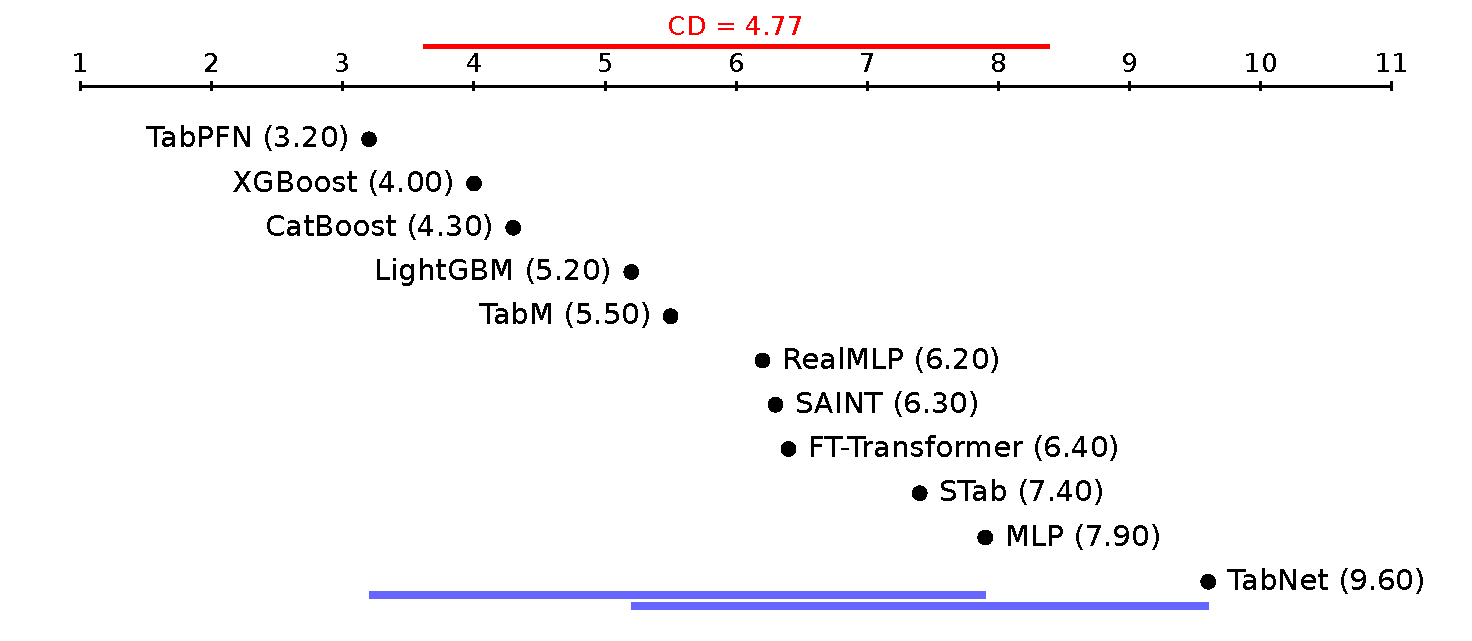
\includegraphics[width=0.9\linewidth]{images/cd_diagram_binary_11.pdf}
\caption[Critical-difference diagram, 11-model core]{Nemenyi
critical-difference diagram for binary classification on the
11-model core ($N{=}10$, $\mathrm{CD}=4.77$). The top bar connects
TabPFN to the MLP: the post-hoc does not separate the pack, which is
why the equivalence reading uses the Bayesian instrument.}
\label{fig:cap5-cd}
\end{figure}

\begin{figure}[htb]
\centering
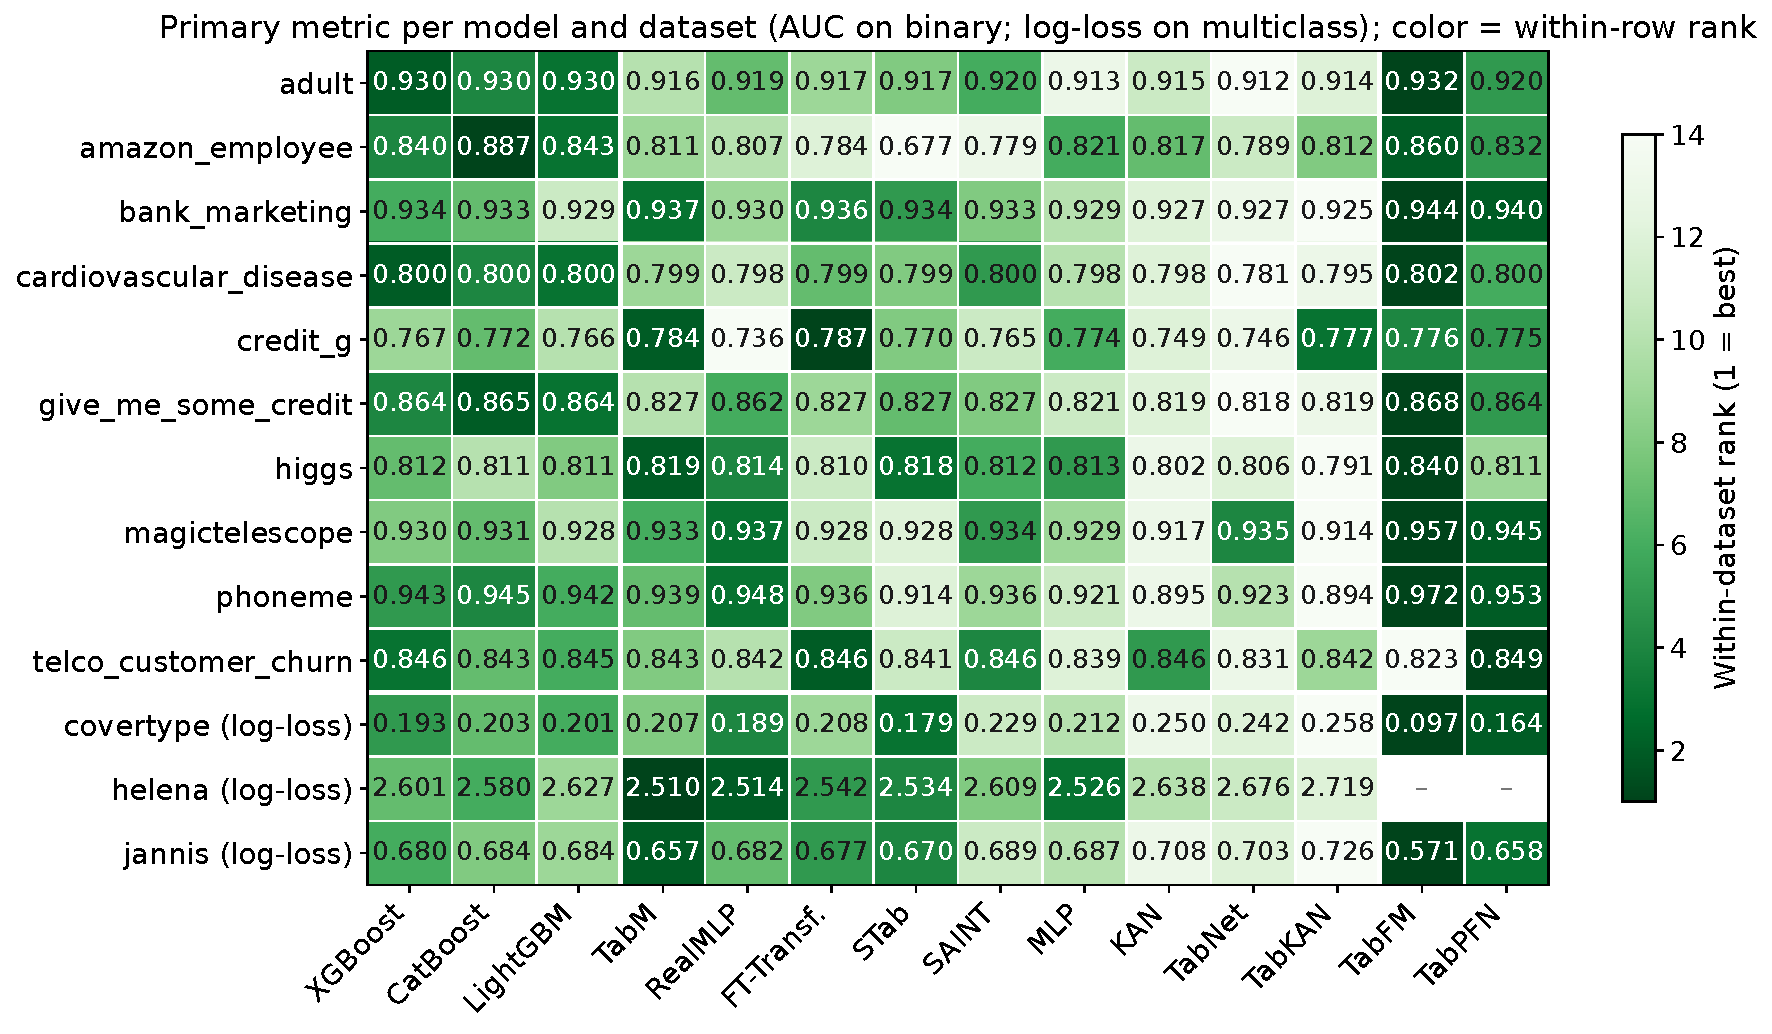
\includegraphics[width=\linewidth]{images/heatmap_classification_en.pdf}
\caption[Primary metric per model and dataset]{Primary metric per
model and classification dataset (AUC on binary, log-loss on
multiclass); color encodes the within-dataset rank (darker =
better). Empty cells: structural exclusions
(\texttt{helena}~$\times$~FMs).}
\label{fig:cap5-heatmap}
\end{figure}

\section{Cost axes: training, tuning, latency}
\label{sec:cap5-custos}

Accuracy near-ties make cost the deciding axis.
\textbf{Training}: median fit time over the 18 datasets --- 17 for
TabPFN --- spans ${\sim}300\times$ (LightGBM 0.66~s, XGBoost 0.69~s,
TabPFN 1.35~s at one forward pass, against ${\sim}200$~s for
SAINT/STab-class deep models). \textbf{Tuning}: GBDTs complete their
100-trial search in 104--646~s; deep models pay up to 14{,}622~s
(STab) --- a $140\times$ spread --- while the in-context models pay
zero by construction. \textbf{Inference latency} (amortized batch,
each model on its natural device, measured on \texttt{adult}):
XGBoost serves at 0.33~\us/row, TabPFN at 7{,}416, TabFM at 43{,}262
--- about five orders of magnitude for TabFM
($\approx131{,}000\times$), with the ratio varying by dataset
(full per-model costs in the appendix).
Figure~\ref{fig:cap5-pareto} folds accuracy and cost into Pareto
fronts: on the core, \{TabPFN, XGBoost, LightGBM\} on the
training-cost axis, narrowing to \{XGBoost, TabPFN\} on latency; on
the full grid the front becomes \{XGBoost, TabPFN, TabFM\}, with the
foundation models paying four to five orders of magnitude of latency
for the rank.

\begin{figure}[htb]
\centering
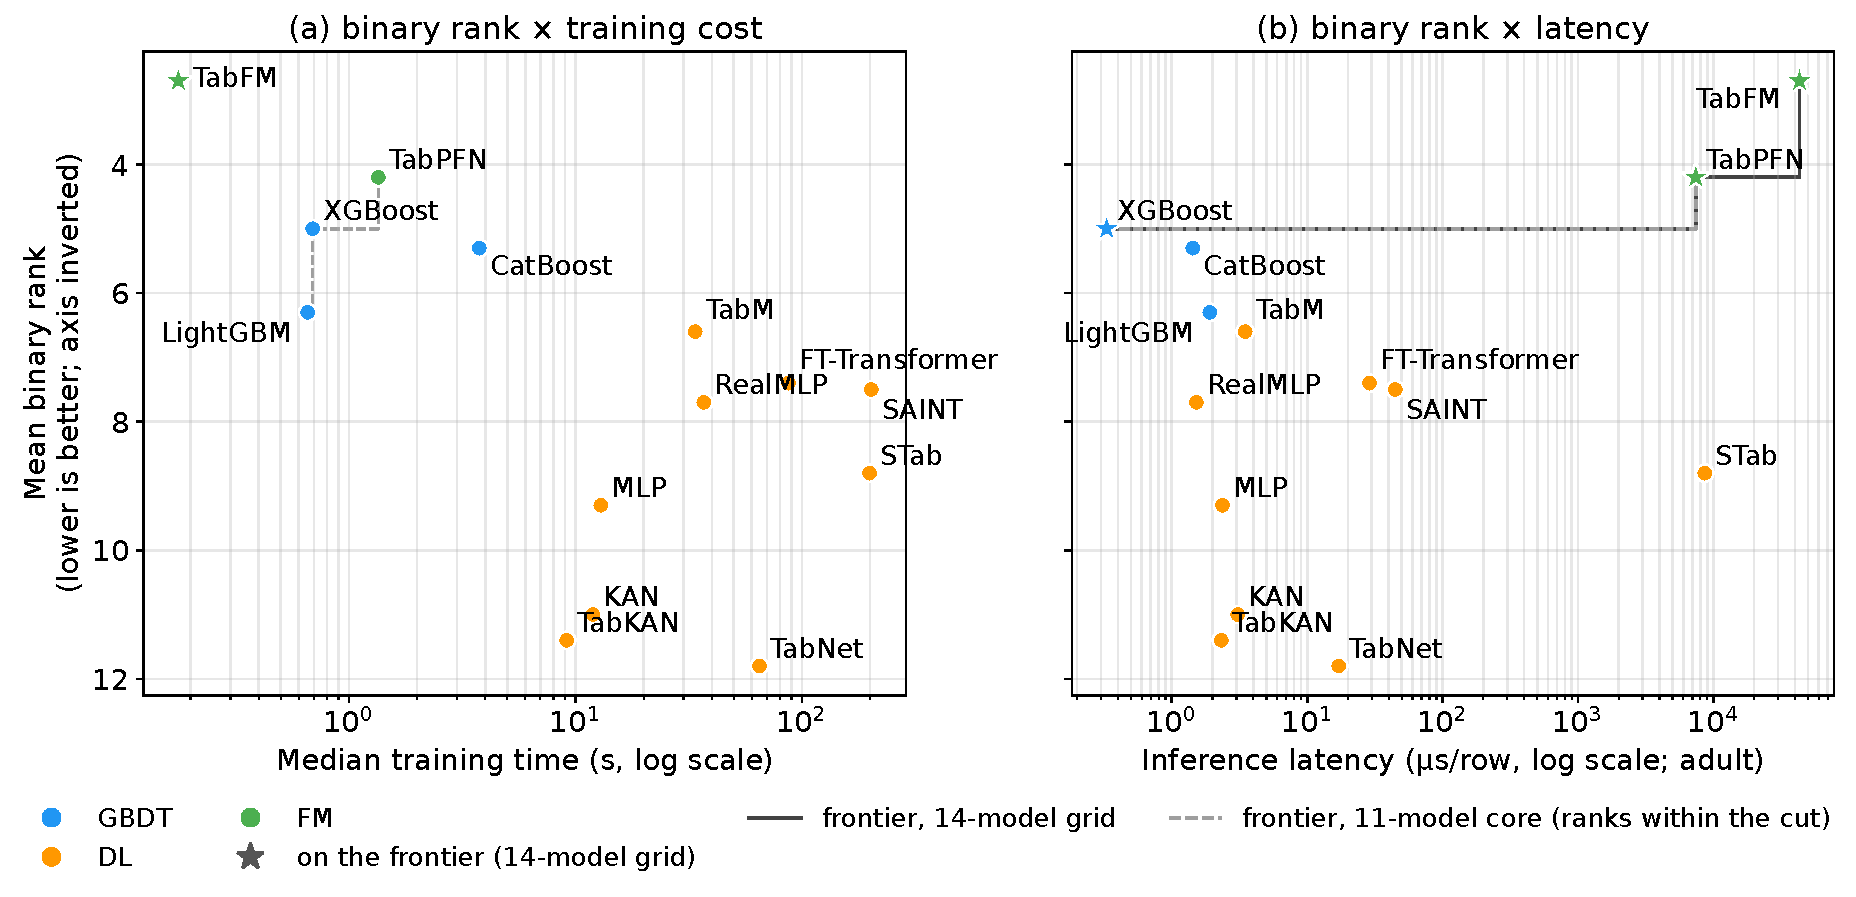
\includegraphics[width=\linewidth]{images/pareto_binary_en.pdf}
\caption[Accuracy--cost Pareto fronts]{Mean binary rank against
median training time (left) and inference latency (right), full
14-model grid; stars mark the Pareto front.}
\label{fig:cap5-pareto}
\end{figure}

\section{Conditional reversals: imbalance and sample size}
\label{sec:cap5-reversals}

Leadership is conditional on regime. Under class imbalance the GBDTs
\emph{gain} ground as severity grows (mean rank 6.6 in the mild
band, 5.5 moderate, 4.6 severe) while tabular deep learning loses it
(8.7/8.9/9.6); the foundation models stay ahead in every band
(3.3/4.1/2.7). On the sample-size axis, learning curves on five
datasets (500 samples to the full pool,
Figure~\ref{fig:cap5-curvas}) show the GBDT$\leftrightarrow$DL
crossover is real and dataset-specific --- deep learning overtakes
for good on 3 of 5 (2 of 4 setting aside
\texttt{year\_\allowbreak prediction}, whose DL curves reflect the
unstandardized target), while on \texttt{adult} the GBDT takes the
lead at $n \approx 4{,}000$ --- and TabPFN has the best
regime-averaged metric on all five swept datasets for
$n \leq 4{,}000$: the zero-shot paradigm is strongest exactly where
data are scarce.

\begin{figure}[htb]
\centering
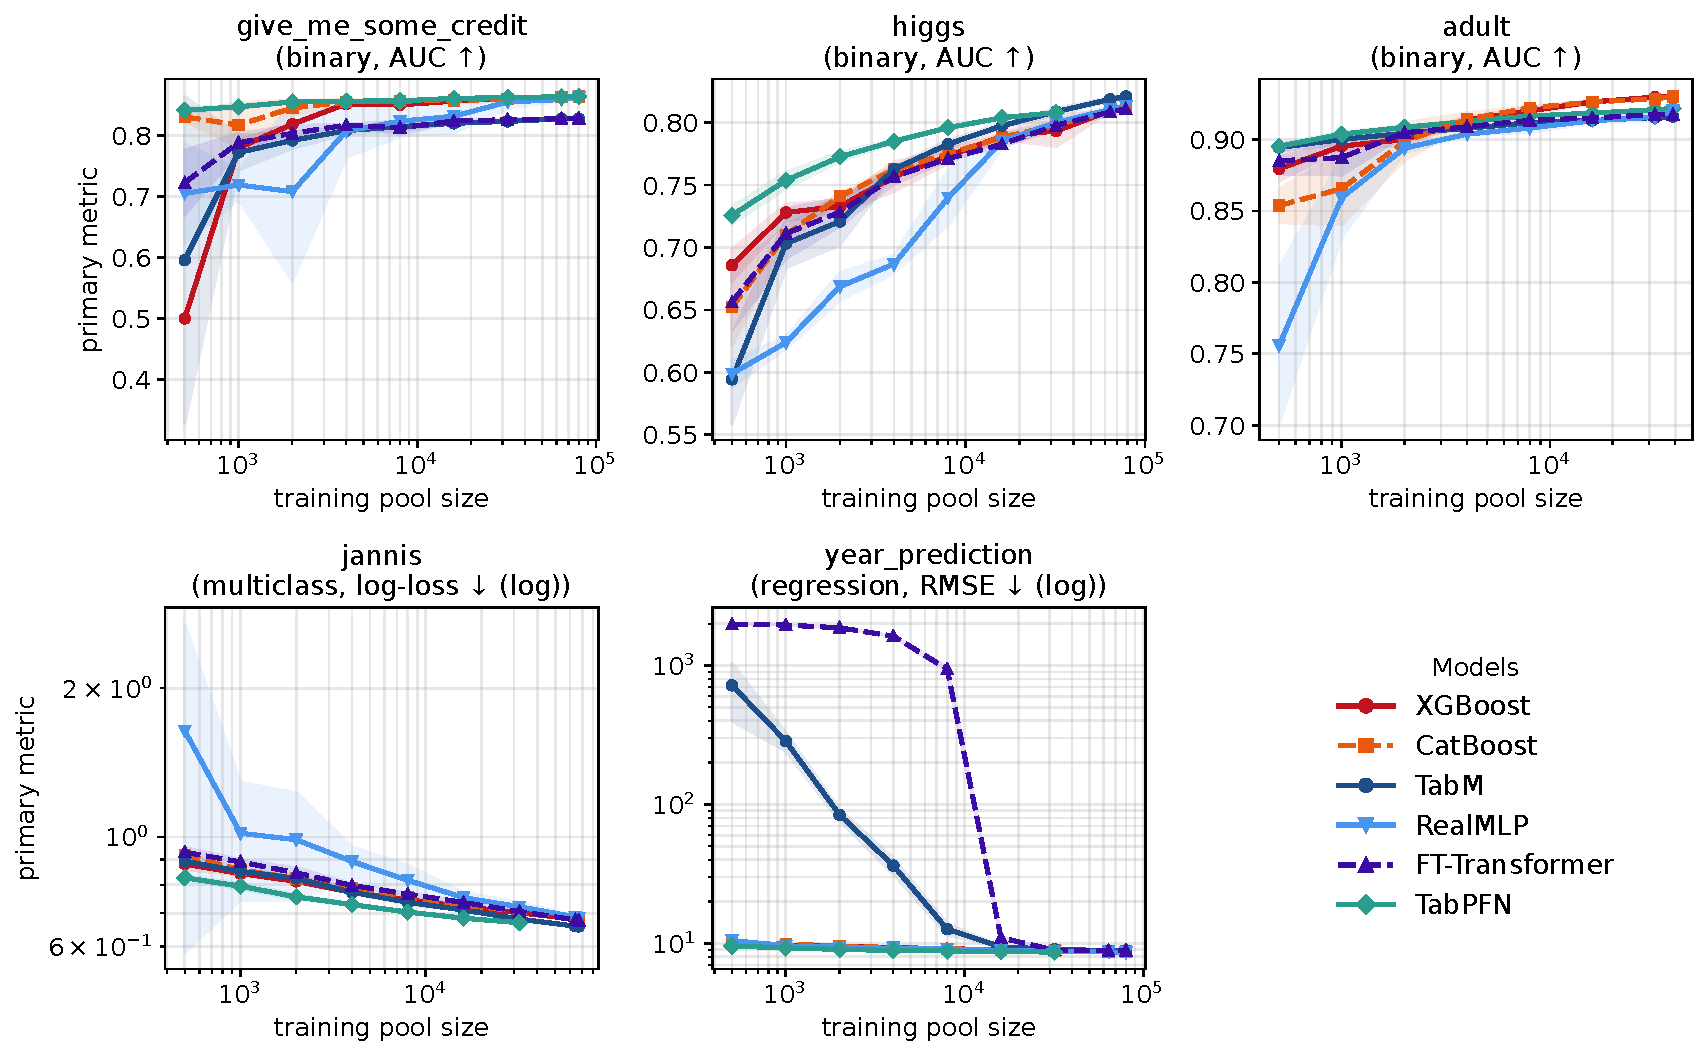
\includegraphics[width=\linewidth]{images/learning_curves_diss_en.pdf}
\caption[Learning curves on five datasets]{Primary metric against
training-set size (log), five datasets $\times$ six models, 3 seeds
(bands: $\pm1$ sd). The last panel carries the legend.}
\label{fig:cap5-curvas}
\end{figure}

\section{The 2026 generation shifts the top}
\label{sec:cap5-shift}

Extending the grid with the 2026 entrants (TabFM; KAN and TabKAN as
the Kolmogorov--Arnold representatives) changes the leadership
without rejecting the tie. Zero-shot TabFM leads the mean rank in
all three tasks (Table~\ref{tab:cap5-ranks}; in multiclass, over the
two datasets where it operates --- \texttt{helena}'s 100 classes are
a structural exclusion for both FMs) and is the single best model on
13 of the 18 datasets (operating on 17). The lead is consistent
across datasets, but no test confirms it as a statistical
separation: with $k{=}14$ the critical distance grows to 6.27 and
the underpowered post-hoc separates nothing; the paired effect size
against XGBoost is $d = 0.68$; and the Bayesian instrument puts 0.67
of the posterior on TabFM's superiority over XGBoost (0.33 on
equivalence; $E[\theta] = 0.40$), with equivalence modal against
CatBoost. In regression, $N{=}5$ puts the Wilcoxon floor at 0.0625
--- a combinatorial floor; multiclass ($N{=}3$) and regression
readings are descriptive. The Kolmogorov--Arnold family lands in the
bottom third on every task (KAN 11.0/12.0/9.8; TabKAN
11.4/13.3/11.8, behind even TabNet in multiclass and regression) ---
an informative negative, with the caveat that both are
reimplementations under a uniform protocol.

\begin{table}[htb]
\centering
\caption[Mean ranks per task, full grid]{Mean rank per task on the
full 14-model grid (lower is better; multiclass over the datasets
each model runs on). Full 14-row table in the extended report.}
\label{tab:cap5-ranks}
\begin{tabular}{lccc}
\toprule
 & Binary & Multiclass & Regression \\
\midrule
\textbf{TabFM}      & \textbf{2.7} & \textbf{1.00} & \textbf{1.2} \\
TabPFN              & 4.2          & 2.50          & 3.0 \\
Best non-FM         & XGBoost 5.0  & STab/TabM 3.67 & XGBoost 5.0 \\
KAN                 & 11.0         & 12.0          & 9.8 \\
TabKAN              & 11.4         & 13.3          & 11.8 \\
\bottomrule
\end{tabular}
\end{table}

\section{Instance-level complementarity}
\label{sec:cap5-ato5}

Where do the foundation models and XGBoost disagree? A sanity gate
first reproduces the benchmark's cells from stored predictions (52
cells, 51 exact and 1 within $6\times10^{-6}$), then per-instance
agreement is measured on the classification hold-outs: the FMs and
XGBoost agree on 93.6--95.0\% of instances, leaving a disputed
\emph{fringe} of 0.6--15.5\% per dataset. Inside the fringe the
asymmetry is strong and dataset-dependent: McNemar rejects the tie
at 1\% in 14 of 24 model$\times$dataset cells, with a median balance
of $+6.6$ net FM wins per 1{,}000 instances
(Figure~\ref{fig:cap5-compl}); TabFM converts the fringe
overwhelmingly on some datasets and \emph{loses} it on
\texttt{telco\_\allowbreak customer\_\allowbreak churn} --- the
dataset where Chapter~\ref{chap:metodologia}'s declared
preprocessing idiosyncrasy penalizes only the FM (0.8233 raw against
0.8515 with numeric \texttt{TotalCharges}), so that cell reads as a
pipeline artifact, not a model property. The two registered
mechanistic hypotheses are not confirmed at 5\%: FM gains
concentrate in minority-class instances on 7/10 datasets ($p=0.17$)
and in low-XGBoost-confidence instances on 8/10 ($p=0.055$). On
\texttt{amazon\_\allowbreak employee} (5.8\% minority) the practical
reading is sharp: near-identical accuracies (${\sim}94.3\%$) hide
minority recalls of 0.032 (XGBoost), 0.214 (TabPFN) and 0.298
(TabFM) at the 0.5 threshold --- when the minority class is what the
application pays for, the FMs' advantage is operational, not
cosmetic.

\begin{figure}[htb]
\centering
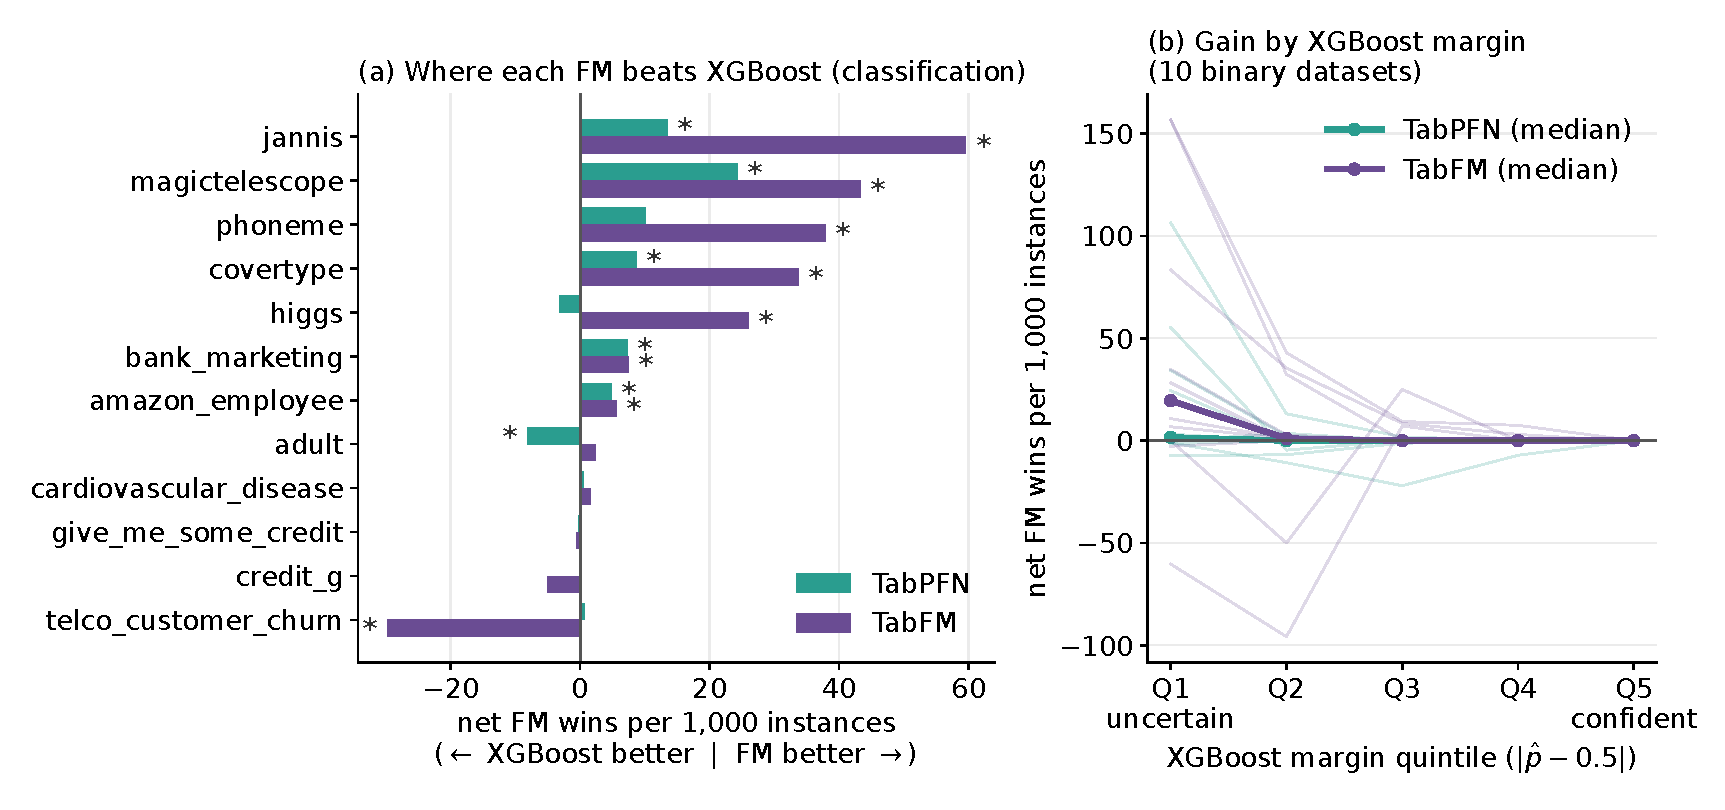
\includegraphics[width=\linewidth]{images/complementarity_diss_en.pdf}
\caption[Instance-level complementarity]{Net FM wins per 1{,}000
instances against XGBoost per dataset (left; $*$ = McNemar at 1\%)
and gain by XGBoost-margin quintile (right).}
\label{fig:cap5-compl}
\end{figure}

\section{Summary: the answer to RQ1}
\label{sec:cap5-sintese}

\emph{Within the pre-2026 core, the top of binary accuracy is a
statistical tie that includes a foundation model as leader; costs,
not accuracy, separate the models. The 2026 generation shifts the
top --- TabFM leads every task's mean rank and wins 13 of 18
datasets zero-shot --- without that tie ever being rejected by an
underpowered post-hoc or by the Bayesian instrument, and at the
price of about five orders of magnitude of serving latency on the
reference dataset. Leadership is conditional (imbalance, sample
size), and the per-instance layer shows where the FM advantage is
operational. The practical question moves from ``which family wins''
to ``which constraints decide'' --- Chapter~\ref{chap:framework}.}

%% Condensed from dissertacao-en/chapters/cap6-framework.tex @295dde3.
\chapter{The Decision Framework, Evaluated}
\label{chap:framework}

If accuracy near-ties and costs decide, how should a practitioner
choose? This chapter submits the decision framework to evaluation by
three studies on the benchmark's own datasets (18; 17 where the FM
family participates): a negative result on learned routing, a
positive result on a fixed-policy reading, and a registered
weighted-regret analysis that locates when the recommendation
flips. Full tables and the multi-criteria star matrix are in the
extended report.

\section{Regret and the LODO protocol}
\label{sec:cap6-regret}

Normalized regret measures, per dataset, how far a choice sits from
that dataset's best model on the primary metric, scaled to $[0,1]$
(on \texttt{adult}, picking the best GBDT costs regret 0.10; the
best deep model, 0.60). Policies are evaluated under
leave-one-dataset-out (LODO) where learning is involved: the router
is trained on 17 datasets and judged on the held-out one --- the
most rigorous protocol available at $N{=}18$.

\section{A negative and a positive result}
\label{sec:cap6-router}

\textbf{Routing by meta-features does not generalize.} A
decision-tree router over dataset meta-features hits the correct
model family on 0.11 of held-out datasets against 0.44 for the
trivial rule ``always predict the most frequent family'' with 11
models, and 0.72 against 0.78 with 14 (including the 2026
generation); a registered robustness sweep over eight router
configurations leaves the conclusion unchanged in every cell. The
most likely cause is structural: each LODO round trains on 17
examples, a sample where any partition by meta-features is dominated
by the noise of individual reversals.

\textbf{A fixed policy is regret-optimal.}
Table~\ref{tab:regret-lodo} evaluates fixed policies descriptively
(only the tree is a learned object under LODO; ``Always-FM'' is the
within-family oracle --- the family's ceiling). At 14 models the
oracle has median regret 0.000 and mean 0.021; the \emph{executable}
always-TabFM also has median 0.000 with mean 0.080, pulled by a
single worst case of 1.000 on
\texttt{telco\_\allowbreak customer\_\allowbreak churn} --- the
dataset whose declared preprocessing idiosyncrasy penalizes the FM
(Chapter~\ref{chap:metodologia}); always-TabPFN sits at median 0.242.
By the mean, the LODO tree (0.051) beats every executable fixed
policy --- the headline ``FM first'' is a median statement about a
family ceiling, and the chapter says so wherever it is used.

\begin{table}[htb]
\centering
\caption[Normalized regret of policies under LODO]{Mean and median
normalized regret of the LODO tree and fixed policies, at 11 and at
14 models. ``Always-FM'' is the within-family oracle; the executable
policies are listed separately.}
\label{tab:regret-lodo}
\small
\begin{tabular}{lcccc}
\toprule
Policy & mean @11 & median @11 & mean @14 & median @14 \\
\midrule
Tree (LODO)        & 0.228 & 0.145 & 0.051 & 0.000 \\
Always-GBDT        & 0.249 & 0.168 & 0.305 & 0.291 \\
Always-DL          & 0.189 & 0.132 & 0.313 & 0.349 \\
\textbf{Always-FM} & \textbf{0.115} & \textbf{0.018} & \textbf{0.021} &
\textbf{0.000} \\
\midrule
Always-TabFM (executable)  & --- & --- & 0.080 & 0.000 \\
Always-TabPFN (executable) & 0.115 & 0.018 & 0.261 & 0.242 \\
\bottomrule
\end{tabular}
\end{table}

\section{When the recommendation flips: weighted regret (E2)}
\label{sec:regret-ponderado}
\label{sec:e2-resultados}

E2 is a \emph{registered analysis} (design fixed before execution;
not a pre-registration, since the accuracy-only endpoint was already
known): the per-dataset score becomes
$S = w \cdot r_{\mathrm{acc}} + (1-w) \cdot r_{\mathrm{lat}}$, with
rank-normalized accuracy and latency, swept over $w$
(Figure~\ref{fig:cap6-regret}). ``FM first'' is regret-optimal by
the median only while $w \geq 0.9$: shifting \textbf{10--20\%} of
the weight from accuracy to latency hands the lead to the cheaper
families (by the mean, 20--30\%). The band is a property of the
design's rank normalization: min--max alternatives move the flip to
20--25\% (logarithmic) and 30--35\% (linear) --- the direction is
the same, and the rank normalization flips earliest. The latency
proxy was also stress-tested: re-running the sweep with latency
measured on a small and a large dataset leaves the crossover
identical, with the always-GBDT zone shifting $\pm0.1$ --- in the
direction opposite to the one anticipated in the record.

\begin{figure}[htb]
\centering
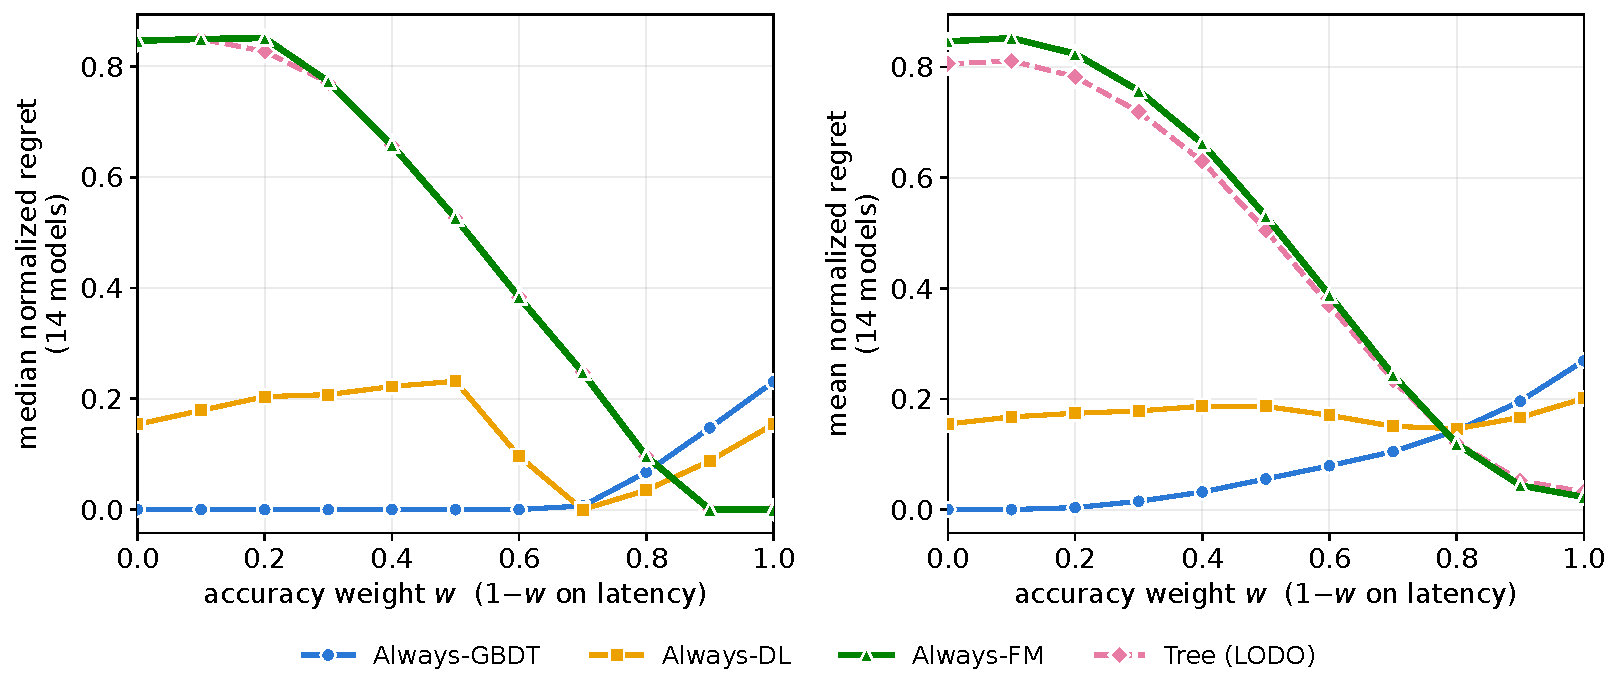
\includegraphics[width=\linewidth]{images/lodo_weighted_regret.pdf}
\caption[Weighted regret against the latency weight]{Median (left)
and mean (right) normalized regret of the policies as the weight
moves from accuracy ($w{=}1$) to latency.}
\label{fig:cap6-regret}
\end{figure}

\section{The resulting framework: decision by constraints}
\label{sec:arcabouco-resultante}

The three studies justify a constraint-first flowchart
(Figure~\ref{fig:cap6-flow}): latency budget, architectural limits
(>10 classes; context caps), and the requirement of auditable
explanations --- GBDTs are accepted in regulated practice via
attribution-based explanations, which is an acceptance criterion,
not strict intrinsic interpretability --- are checked in order;
with no active constraint, foundation model first (TabPFN mature;
TabFM frontier, v1.0.1 caveats). The flowchart is a \emph{synthesis
of the three studies, not an evaluated policy}: no end-to-end
accuracy claim is attached to following it.

\begin{figure}[htb]
\centering
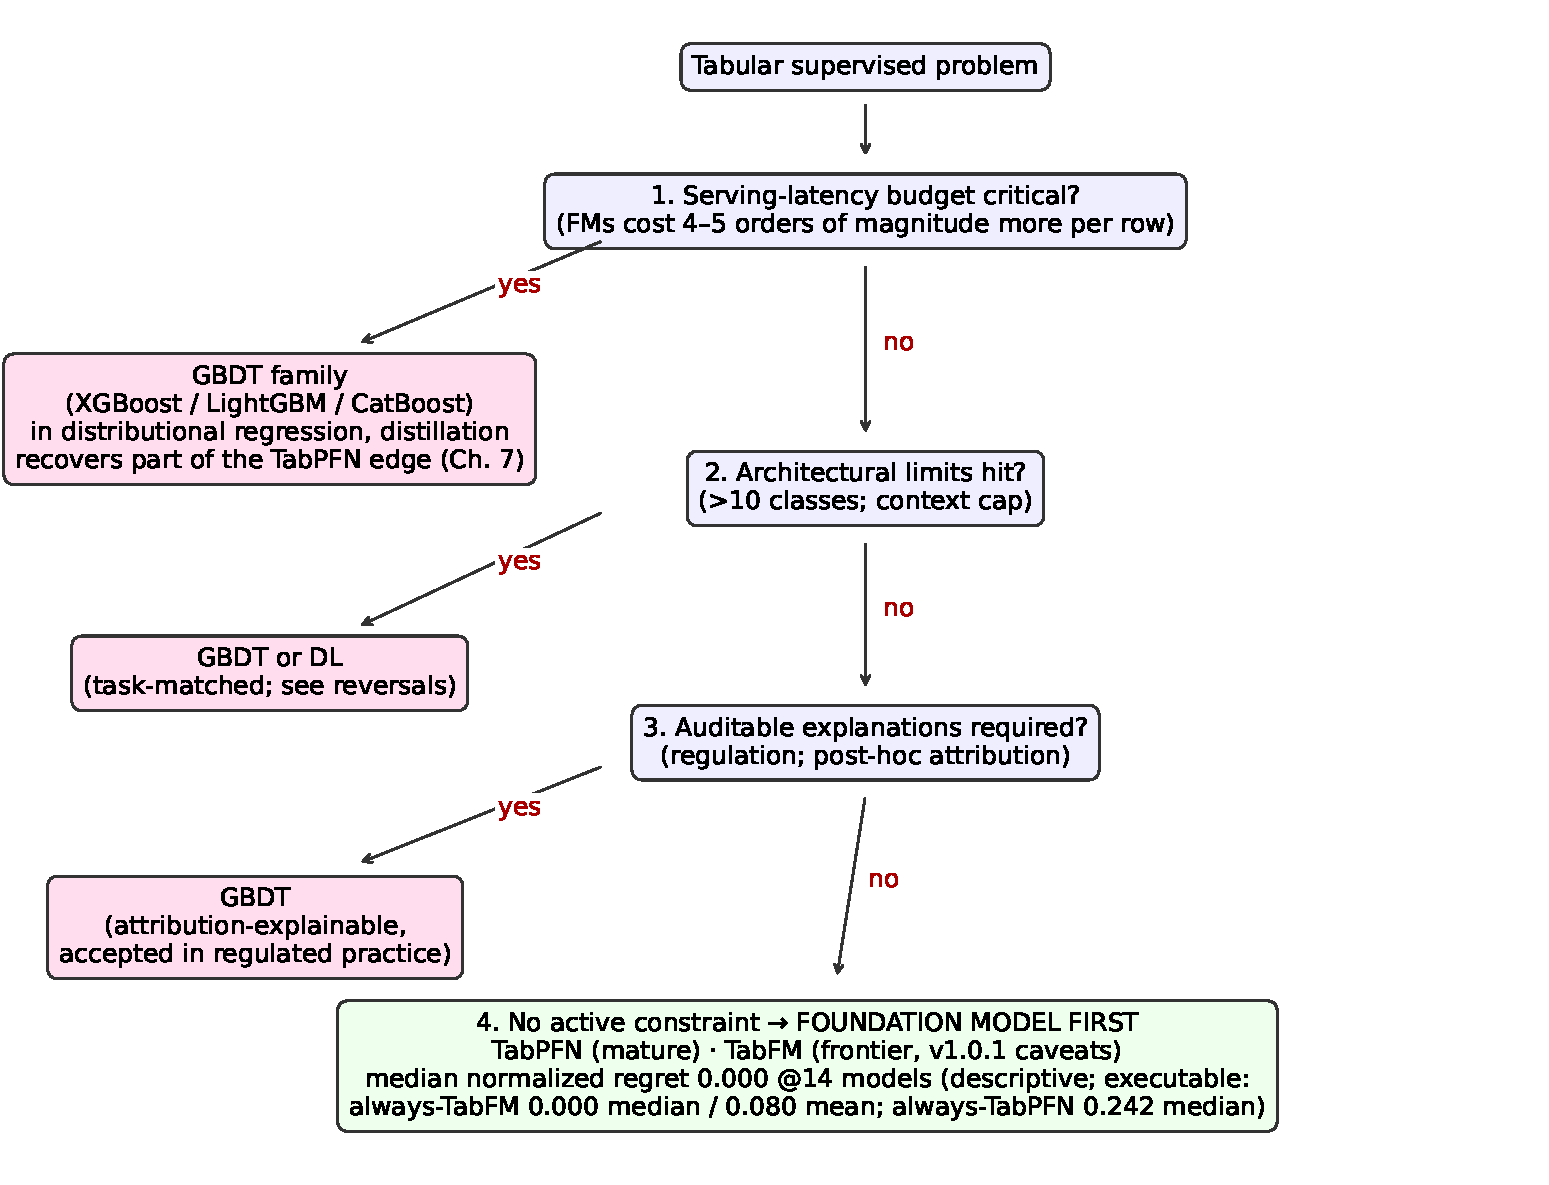
\includegraphics[width=0.9\linewidth]{images/decision_flowchart_14_en.pdf}
\caption[The evaluated decision flowchart]{The four-constraint
flowchart at 14 models. Each box is a constraint verifiable a
priori.}
\label{fig:cap6-flow}
\end{figure}

\emph{Limitations, briefly: regret compares models within this
benchmark's grid; the flip band depends on the score normalization
(10--20\% by ranks; up to 35\% under min--max variants); latency
enters by a single-machine proxy; only the tree was evaluated under
LODO; and the flowchart inherits every caveat of
Chapter~\ref{chap:benchmark}'s measurements.}

%% Condensed from dissertacao-en/chapters/cap7-destilacao.tex @295dde3.
%% Every number and qualifier exists in the extended report (same chapter).
\chapter{Distributional Distillation}
\label{chap:destilacao}

The benchmark's accuracy leader costs four to five orders of
magnitude more latency per row than a gradient-boosted tree. This
chapter asks what of a tabular foundation model's advantage can be
carried into a student that serves fast --- and answers RQ3 with a
selective result: \emph{point} distillation does not transfer,
\emph{distributional} distillation transfers a modest, measurable
part, and the conditions under which it is worth doing can be
checked before training the student. Full process record, ablation
tables and per-run artifacts are in the extended technical report
and in the project repository.

\section{Question and setup}
\label{sec:destil-setup}

\textbf{Teacher.} TabPFN-2.5 \citep{hollmann2025,priorlabs2025}, an
8-member ensemble with the training context capped at 50{,}000 rows,
re-labels each dataset's training pool \emph{out-of-fold} (OOF): the
pool is split into folds, and each fold receives predictions from a
teacher whose context excludes it. The teacher natively outputs a
predictive distribution, read as 19 quantile curves
($\tau \in \{0.05, \ldots, 0.95\}$). TabFM cannot play this role:
its regression head is point-valued (an architectural negative
confirmed by the official technical report, \citealp{kong2026});
Section~\ref{sec:destil-ponto} uses it as a point-teacher anchor.

\textbf{Students and control.} The distilled student is the
benchmark's XGBoost with a 19-output head trained by squared error
on the teacher's quantile curves; the \emph{control} is the same
architecture trained by pinball loss on the true labels --- so the
teacher is the only difference between the arms. A point student
(single output, trained on the teacher's means) answers H1, and a
true-label quantile MLP enters the decision rule's analysis. All
students inherit the benchmark's tuned hyperparameters; the
re-tuning analysis below removes that crutch.
Figure~\ref{fig:destil-pipeline} summarizes the pipeline.

\begin{figure}[htb]
\centering
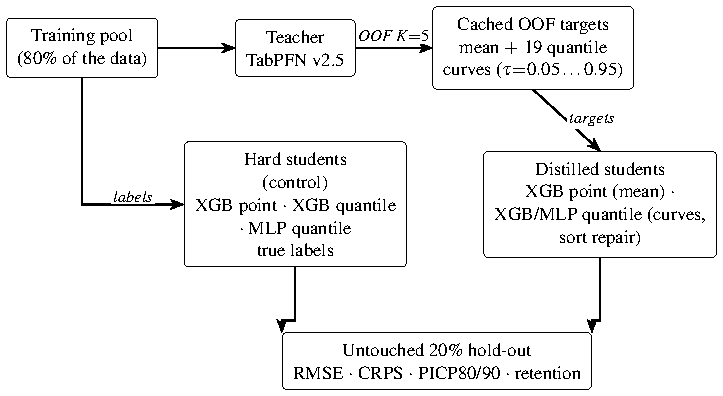
\includegraphics{images/tikz-cap7-1-en.pdf}
\caption[Distributional distillation pipeline]{Distributional
distillation pipeline: the teacher labels the pool OOF with 19
quantile curves; the distilled student regresses on the curves; the
control learns the same quantiles from the true labels. Source: the
author.}
\label{fig:destil-pipeline}
\end{figure}

\textbf{Metric.} Quality is CRPS on the untouched hold-out,
estimated from the 19 quantiles. The headline quantity is
\emph{retention}: the fraction of the teacher's CRPS advantage over
the control that the distilled student preserves,
$(\mathrm{CRPS}_{\mathrm{ctrl}} -
\mathrm{CRPS}_{\mathrm{dist}})/(\mathrm{CRPS}_{\mathrm{ctrl}} -
\mathrm{CRPS}_{\mathrm{teach}})$. On \texttt{cpu\_activity}, for
example, the control scores 1.294, the teacher 1.061 and the
distilled student 1.178: the student recovers half of the gap
(retention $+0.500$), a 9.0\% CRPS gain over the control.

\textbf{Datasets.} 20 regression datasets: the 5 central ones plus
15 from the OpenML-CTR23 suite. Four eligible CTR23 datasets were
left out of the extension (one with no recorded justification); a
sensitivity run on five data splits puts the scoreboard with them at
17/24 ($p=0.032$), and excluding the two datasets that overlap the
teacher's pre-training corpus gives 16/22 ($p=0.026$) --- the
verdict does not depend on the roster choice.

\section{Registered design}
\label{sec:destil-desenho}

The design was registered in two stages: the July~15 pre-registration
fixed H1--H3 on the five central datasets before any execution; the
confirmatory sign test and the extension's eligibility rule were
fixed at an interim reading (11/15, $p=0.059$), and the final test
therefore carries a two-stage sequential correction --- the headline
$p=0.006$ is reported as $p\approx0.019$ after splitting the
significance level across the two looks (single-stage threshold
0.0118). Table~\ref{tab:destil-hipoteses} lists every hypothesis and
analysis with its registration status and verdict; negative results
are reported with the same prominence as positive ones.

\begin{table}[htb]
\centering
\caption[The chapter's hypotheses and registration status]{The
chapter's hypotheses and analyses: what each claims, whether it was
fixed before any reading of results, and the verdict. Dates and full
records in the extended report.}
\label{tab:destil-hipoteses}
\small
\begin{tabular}{>{\raggedright\arraybackslash}p{0.14\linewidth}>{\raggedright\arraybackslash}p{0.35\linewidth}>{\raggedright\arraybackslash}p{0.18\linewidth}>{\raggedright\arraybackslash}p{0.21\linewidth}}
\toprule
Code & What it claims & Before reading? & Verdict \\
\midrule
H1 (point) & point student retains $\geq$50\% of the RMSE gap on
$\geq$3/5 & yes & refuted (0/5 central datasets reach 50\%
retention; descriptively, it beats the control on 4/20) \\
\addlinespace[2pt]
H2 (distribution) & distilled beats the control in CRPS, with
coverage within $\pm$5~p.p. & yes & not confirmed as a conjunction:
CRPS clause sustained (16/20); coverage clause not met (10/20) \\
\addlinespace[2pt]
H3 (Pareto) & there is a latency band where the distilled student
dominates the compressed teacher & yes & not confirmed as
registered: dominance only on \texttt{year}, at 169~\us{} (above
the ${\lesssim}100$ band); within the band, merely non-dominated,
and only on california$^\dagger$; refuted on \texttt{kin8nm} \\
\addlinespace[2pt]
Sign test & confirmatory instrument of the 16/20 & no (fixed at the
interim reading) & $p\approx0.019$ sequential \\
\addlinespace[2pt]
Heavy tail (log) & redoing teacher and students with
$y'{=}\log(1{+}y)$ recovers retention on the price-scale failures &
no (fixed at the interim reading, before the ablation) & refuted
(\texttt{fifa} goes from $-1.29$ to $-1.69$ in the transformed
space; the two controls move in opposite directions) \\
\addlinespace[2pt]
E1 (classical) & distilled beats the best of QRF and NGBoost & yes
(execution already started) & confirmed (17/20) \\
\addlinespace[2pt]
E3 (utility) & realized cost lower or equal at $\tau{=}0.90$ &
registered (before any reading) & confirmed (18/20) \\
\addlinespace[2pt]
Re-tuning & inherited hyperparameters are a floor on retention &
partially (pilot read before; extension to the 20 registered in a
dated addendum) & refuted (9/20 per dataset; median
0.19$\to$0.12): sign upheld, magnitude reduced \\
\bottomrule
\end{tabular}
\end{table}

\section{Point distillation does not transfer}
\label{sec:destil-ponto}

The first result is the negative the pre-registration committed to
report. Across the 20 datasets, the point student trained on the
teacher's means beats its true-label control on only \textbf{4}; H1
is refuted already on the five central datasets (0/5 reach the
registered 50\% retention). The natural objection --- ``the teacher
was not strong enough'' --- was tested directly by replicating the
experiment with TabFM as teacher on the five central datasets: its
reference advantage is almost $6\times$ TabPFN's on
\texttt{california\_\allowbreak housing}$^\dagger$ (0.028 against
0.005 RMSE), and the negative holds --- with the caveat that this
anchor rests on a single, binarized-target dataset. A pool-size
sweep (caps 800/2{,}000/8{,}000) shows a genuine low-data gain only
on \texttt{wine\_quality} ($\Delta=+0.026$ at $n{=}800$), gone from
$n{=}2{,}000$ on, and on california$^\dagger$ only a marginal
$+0.005$ residue at 2{,}000. At realistic pool sizes, what the
teacher knows about the \emph{mean}, a tuned GBDT learns on its own
from the raw labels.

\section{Distributional distillation transfers part of the advantage}
\label{sec:destil-dist}

The distilled quantile student beats its control in CRPS on
\textbf{16 of 20} datasets (sign test $p=0.006$ single-stage,
$p\approx0.019$ under the sequential correction), with median
retention $+0.19$ and a median CRPS gain of 2.8\% over the control.
Table~\ref{tab:destil-retencao} gives the result per dataset and
Figure~\ref{fig:destil-forest} the same picture with uncertainty:
by bootstrap confidence interval the scoreboard is 12 clear wins, 1
win at the margin, 3 ties with a positive point estimate, 1 tie with
a negative one, and 3 clear defeats. Two supplementary instruments
agree with different firmness: one-sided Wilcoxon $p=0.045$
(two-sided 0.090 would not reject), and the Bayesian signed-rank
analysis assigns probability 0.96 that the positive-retention region
is the most probable one (ROPE $\pm0.05$; expected posterior mass on
it: $E[\theta]=0.70$).

\begin{table}[htb]
\centering
\caption[Distributional distillation result per dataset]{Result per
dataset (mean of 3 seeds), sorted by retention. Gain = relative CRPS
reduction over the control; CI by bootstrap over hold-out rows.
$^\dagger$binarized-target erratum dataset.}
\label{tab:destil-retencao}
\scriptsize
\setlength{\tabcolsep}{4pt}
\begin{tabular}{lrrrrrr}
\toprule
Dataset & CRPS ctrl & CRPS dist & CRPS teach & Gain (\%) & 95\% CI (\%) & Retention \\
\midrule
pumadyn32nh & 0.0130 & 0.0124 & 0.0124 & $+$4.7 & [3.7; 5.7] & $+$1.057 \\
california\_housing$^\dagger$ & 0.1802 & 0.1086 & 0.0691 & $+$39.7 & [37.1; 42.3] & $+$0.644 \\
abalone & 1.154 & 1.098 & 1.060 & $+$4.9 & [3.0; 6.7] & $+$0.595 \\
fps\_benchmark & 0.4651 & 0.3855 & 0.3128 & $+$17.1 & [15.1; 19.0] & $+$0.523 \\
cpu\_activity & 1.294 & 1.178 & 1.061 & $+$9.0 & [6.4; 11.6] & $+$0.500 \\
cps88wages & 160.8 & 160.6 & 160.4 & $+$0.1 & [$-$0.1; 0.3] & $+$0.465 \\
year\_prediction & 4.558 & 4.427 & 4.246 & $+$2.9 & [2.6; 3.2] & $+$0.419 \\
online\_news & 0.4554 & 0.4540 & 0.4497 & $+$0.3 & [0.0; 0.6] & $+$0.255 \\
sarcos & 1.270 & 1.163 & 0.7961 & $+$8.4 & [7.4; 9.4] & $+$0.225 \\
kings\_county & 50{,}516 & 48{,}969 & 43{,}262 & $+$3.1 & [1.5; 4.6] & $+$0.213 \\
grid\_stability & 0.0043 & 0.0038 & 0.0017 & $+$10.3 & [8.6; 12.0] & $+$0.170 \\
kin8nm & 0.0682 & 0.0644 & 0.0380 & $+$5.7 & [4.4; 7.0] & $+$0.128 \\
physiochemical\_protein & 1.785 & 1.736 & 1.212 & $+$2.8 & [1.9; 3.6] & $+$0.086 \\
video\_transcoding & 0.3053 & 0.2974 & 0.2138 & $+$2.6 & [0.1; 5.0] & $+$0.086 \\
space\_ga & 0.0601 & 0.0592 & 0.0488 & $+$1.5 & [$-$0.9; 3.8] & $+$0.078 \\
miami\_housing & 31{,}999 & 31{,}931 & 27{,}882 & $+$0.2 & [$-$1.9; 2.3] & $+$0.016 \\
health\_insurance & 7.273 & 7.311 & 7.122 & $-$0.5 & [$-$1.3; 0.2] & $-$0.255 \\
diamonds\_real & 192.5 & 195.5 & 183.1 & $-$1.5 & [$-$2.4; $-$0.6] & $-$0.315 \\
wine\_quality & 0.3277 & 0.3652 & 0.2891 & $-$11.4 & [$-$14.6; $-$8.5] & $-$0.970 \\
fifa & 2{,}837 & 2{,}893 & 2{,}795 & $-$1.9 & [$-$3.8; $-$0.1] & $-$1.287 \\
\bottomrule
\end{tabular}
\end{table}

\begin{figure}[htb]
\centering
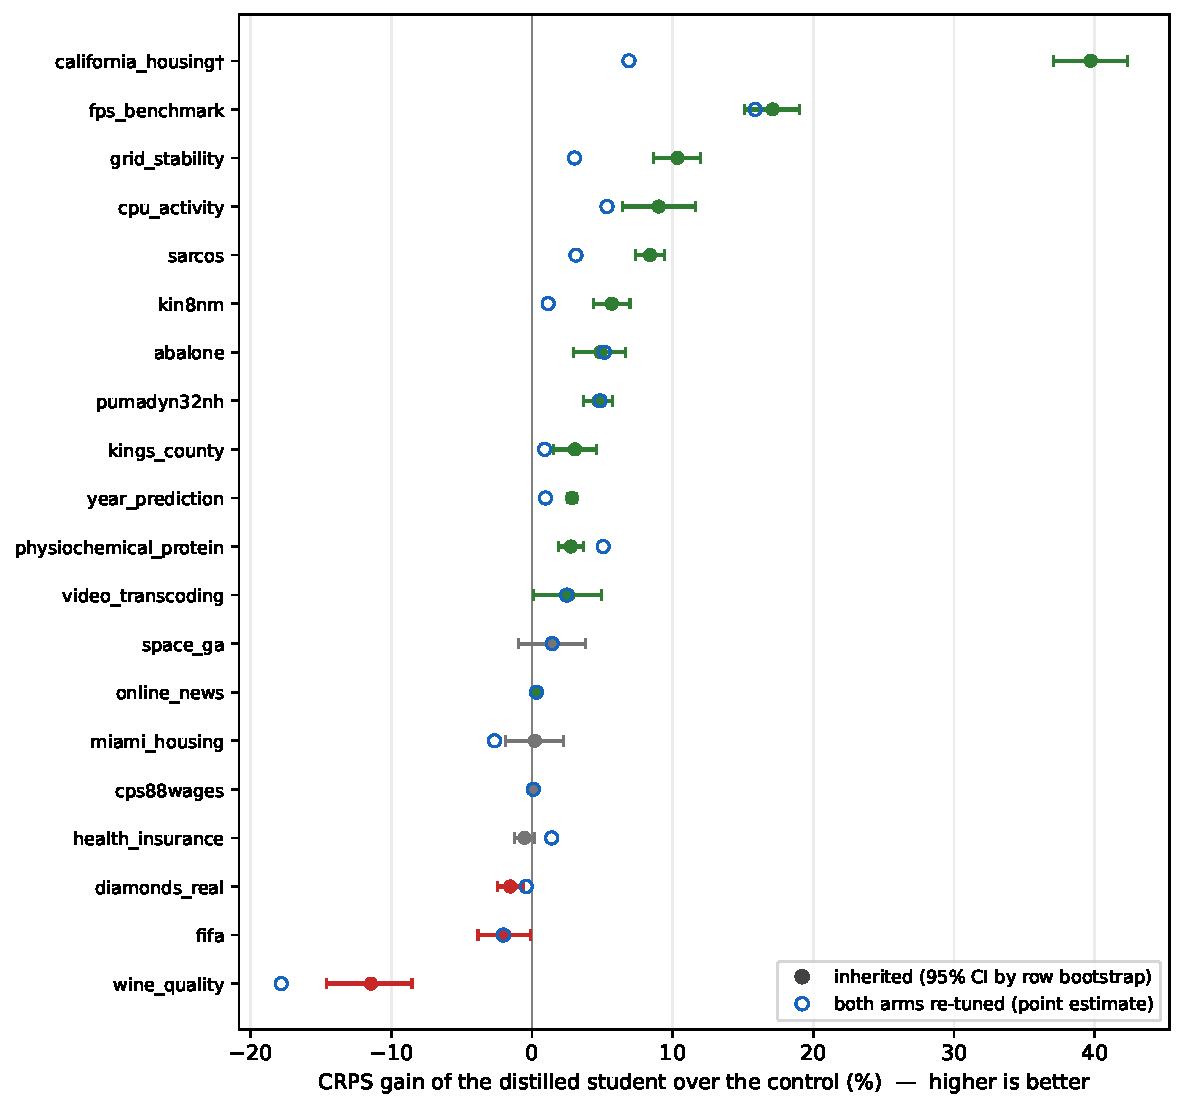
\includegraphics[width=0.92\linewidth]{images/forest_distill_en.pdf}
\caption[CRPS gain per dataset, with uncertainty]{Relative CRPS gain
of the distilled student over the control, with bootstrap 95\% CIs
(log-scaled axis). Source:
\texttt{results/distillation}.}
\label{fig:destil-forest}
\end{figure}

\textbf{Re-tuning: the honest magnitude.} The inherited
hyperparameters were searched for squared error --- the distilled
arm's loss, not the control's. Re-tuning both arms separately
(Optuna, 25 trials each) does not change the scoreboard (16/20,
$p=0.006$; without the binarized dataset 15/19, $p=0.010$) but
halves the magnitude: median retention 0.19$\to$0.12, median CRPS
gain 2.8\%$\to$1.4\% (the re-tuned mean retention is $-0.02$, pulled
by the negatives). The number this work stands behind is therefore a
median CRPS gain of 1.4--2.8\% (retention of 12--19\% of the
teacher's advantage), with the lower end as the conservative
estimate. Table~\ref{tab:destil-robustez} gathers all the
robustness variants.

\begin{table}[htb]
\centering
\caption[Robustness of the distributional distillation verdict]{The
verdict under every variation: roster, re-tuning, seeds and splits.}
\label{tab:destil-robustez}
\small
\setlength{\tabcolsep}{3pt}
\begin{tabular}{lcccc}
\toprule
Variant & Score & Median ret. & Sign (one-s.) & Wilcoxon (one-s.) \\
\midrule
Main (inherited, 3 seeds) & 16/20 & 0.19 & 0.006 (0.019 seq.) & 0.045 \\
Without the binarized & 15/19 & 0.17 & 0.010 & 0.067 \\
Both arms re-tuned & 16/20 & 0.12 & 0.006 & 0.035 \\
Re-tuned, without the binarized & 15/19 & 0.10 & 0.010 & 0.048 \\
Ten student seeds & 16/20 & 0.19 & --- & --- \\
With the 4 omitted eligible (5 splits) & 17/24 & --- & 0.032 & --- \\
Without the 2 overlapping the core (5 splits) & 16/22 & --- & 0.026 & --- \\
\bottomrule
\end{tabular}
\end{table}

\textbf{The defeats are diagnosable.} \texttt{wine\_quality} is a
dataset artifact: 27.6\% of the test set has an exact covariate twin
in the pool (1{,}179 duplicated rows), and on the deduplicated
dataset ($n=5{,}318$, teacher re-labeled OOF) the defeat disappears.
\texttt{health\_\allowbreak insurance} is configuration-sensitive,
not structural: its retention goes from $-0.26$ (inherited) to
$+0.65$ (re-tuned). \texttt{fifa} and
\texttt{diamonds\_\allowbreak real} remain unexplained failures on
price-scale targets --- and the registered heavy-tail hypothesis
(that a $\log(1{+}y)$ re-run would rescue them) was refuted:
\texttt{fifa} goes from $-1.29$ to $-1.69$ in the transformed space,
and the two positive controls move in opposite directions.

\textbf{Coverage: the H2 clause that fails.} The distilled student's
central-interval coverage lands within $\pm5$~p.p.\ of nominal on
only 10 of 20 datasets (2/5 core), so H2 is not confirmed as a
conjunction: the CRPS clause holds (16/20), the coverage clause does
not. Calibration is the dimension to watch, and
Section~\ref{sec:destil-oof} shows where it comes from.

\section{The serving frontier}
\label{sec:destil-fronteira}

To answer H3, accuracy and latency of \emph{all} strategies ---
distill, compress the teacher's context, shrink its ensemble ---
were measured on the same hold-outs of three positive-advantage
datasets (Figure~\ref{fig:destil-pareto}). The distilled student
delivers CRPS 0.109 at 99~\us/row where the teacher's cheapest
configuration needs 245~\us/row for 0.094
(california$^\dagger$), and 4.43 at 169~\us/row where the cheapest
teacher that beats it costs 4{,}576~\us/row ($27\times$ the latency)
on \texttt{year\_\allowbreak prediction}. On \texttt{kin8nm} the
picture inverts, instructively: the teacher's absolute advantage is
small ($+0.030$ CRPS; its relative advantage, 44\%, is among the
largest) and a \emph{single-member} TabPFN delivers CRPS 0.040 at
150~\us/row --- essentially the student's latency --- so ensemble
shrinking, not distillation, is the right lever: a latency case, not
a small-advantage case.

H3's verdict: \textbf{not confirmed as registered}. Pareto dominance
over the subsampled teacher occurs only on
\texttt{year\_\allowbreak prediction}, at 169~\us/row --- above the
pre-registered ${\lesssim}100$~\us/row band; within the band the
student is merely \emph{non-dominated} (no teacher configuration
operates below 245~\us) and only on california$^\dagger$, where its
CRPS is 15.5\% worse than the teacher's cheapest configuration;
without the binarized dataset the band is not met at all; on
\texttt{kin8nm} the hypothesis is refuted. What stands is the
latency reading: where no cheap teacher configuration reaches the
student's tier, the distilled student is the CRPS-optimal
teacher-derived system in that regime. A side finding: shrinking
TabPFN from 8 members to 1 \emph{improved} RMSE on
california$^\dagger$ (0.2521 against 0.2555) at a seventh of the
latency --- ensemble shrinking is an underrated first lever.

\begin{figure}[htb]
\centering
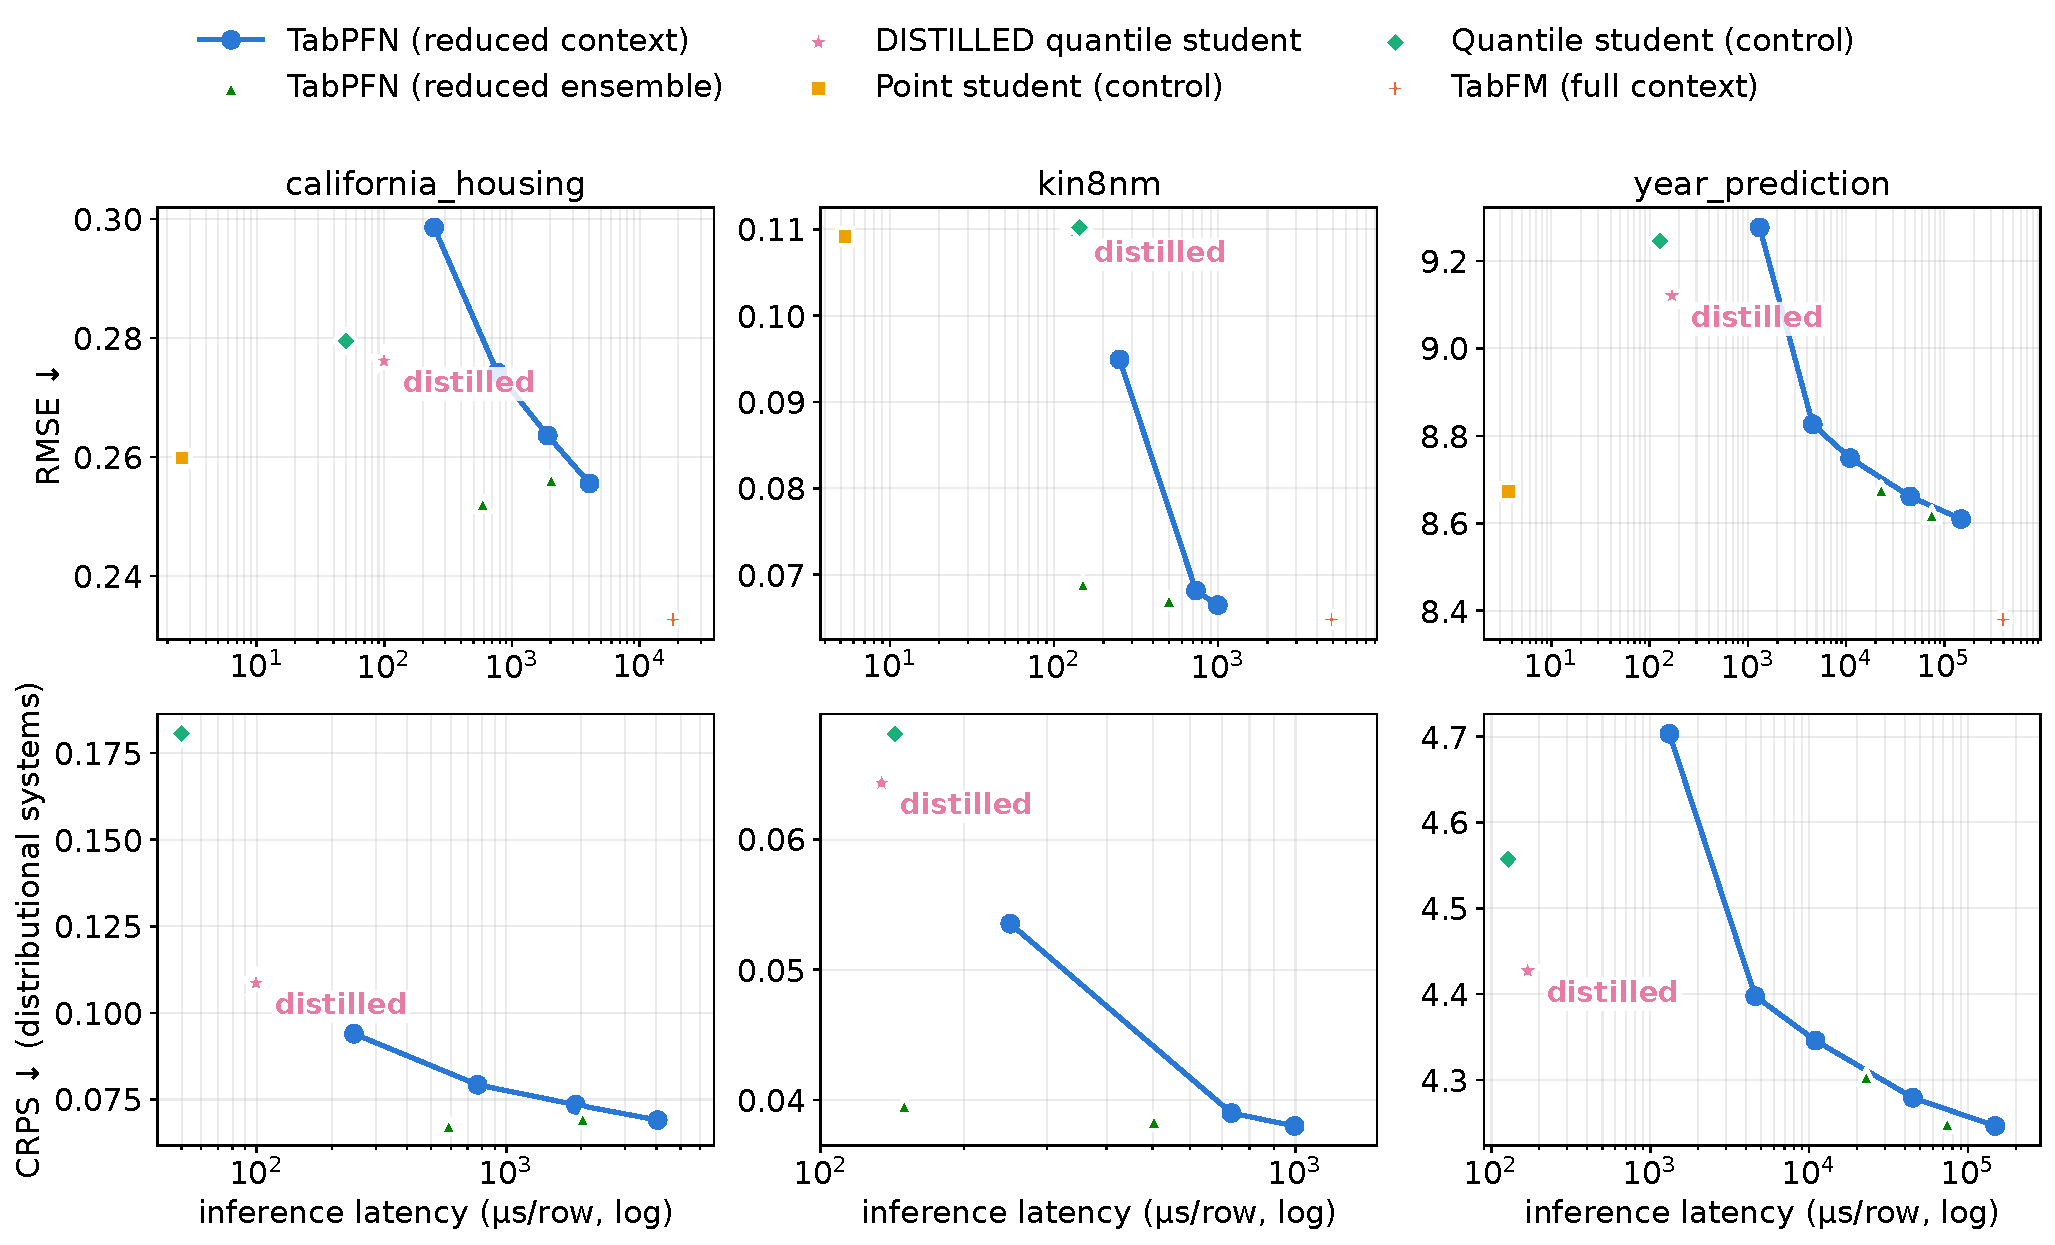
\includegraphics[width=\linewidth]{images/pareto_distill_en.pdf}
\caption[Frontier distill $\times$ compress $\times$ shrink]{The
serving frontier on three datasets: RMSE (top) and CRPS (bottom)
against latency (log). The teacher's context-compression curve, its
shrunk-ensemble points, the distilled student and the controls, with
TabFM (full context) as the accuracy anchor. Source:
\texttt{results/distillation/pareto.csv}.}
\label{fig:destil-pareto}
\end{figure}

\section{OOF labeling protects calibration, not accuracy}
\label{sec:destil-oof}

An ablation relabeling the pool \emph{in-sample} (teacher sees the
rows it labels) moves CRPS by at most ${\sim}0.003$ on three of four
datasets --- and on \texttt{wine\_quality} the in-sample run
\emph{improves} CRPS by 0.029, consistent with the
duplicate-memorization mechanism above. What leakage degrades is
\emph{calibration}: OOF labeling keeps the student's central-interval
coverage 0.5--5.1~p.p.\ closer to nominal. OOF labeling is therefore
the student's calibration safeguard, not an accuracy booster.
Figure~\ref{fig:destil-calibration} shows the hold-out reliability
curves; the reading rule, corrected mid-study, is that the
\emph{slope} decides (steeper than the diagonal = overcoverage) ---
there is no shortcut ``above the diagonal = overcovers''. Two
post-hoc repairs are measured in the extended report: re-sorting the
19 quantile curves repairs 96\% of the crossing violations, and
split-conformal calibration fixes both arms' coverage while leaving
CRPS essentially intact --- distillation and conformalization are
complementary.

\begin{figure}[htb]
\centering
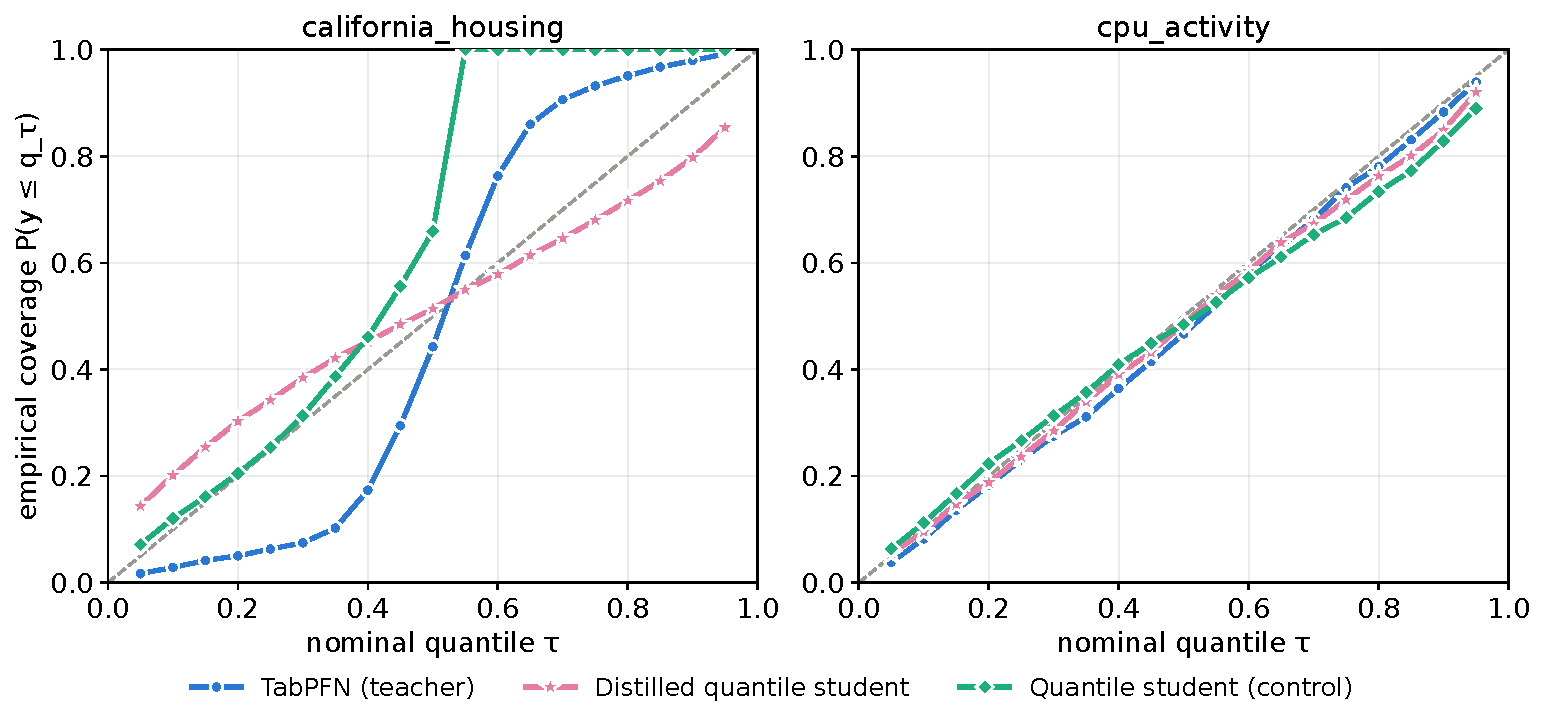
\includegraphics[width=0.9\linewidth]{images/calibration_distill_en.pdf}
\caption[Reliability on the hold-out]{Reliability curves on the
hold-out: empirical coverage $P(y \le q_\tau)$ against nominal
$\tau$, for teacher, distilled student and control, on the
binarized-target california$^\dagger$ (a Bernoulli calibration) and
on \texttt{cpu\_activity}, where the three systems are well
calibrated. Source: \texttt{results/distillation}.}
\label{fig:destil-calibration}
\end{figure}

\section{Classical distributional baselines (E1)}
\label{sec:destil-e1}

Registered question: does the distilled student beat strong
classical baselines that need no teacher at all? Against the best of
Quantile Regression Forest and NGBoost in \emph{default}
configuration, the distilled student wins in CRPS on \textbf{17 of
20} datasets (one-sided sign test $p=0.0013$); against the best
teacher-free alternative chosen \emph{per dataset} by an oracle
(QRF, NGBoost, quantile MLP, or a Gaussian point-plus-residual
baseline), 12 of 20 ($p=0.25$) --- distillation's edge over a
well-chosen native is real but not statistically separable. The
three upsets are diagnosable: on \texttt{wine\_quality} --- flagged
in advance by the registered eligibility criterion --- the default
QRF beats even the teacher; on california$^\dagger$ the QRF (CRPS
0.084) occupies the student's latency band with a better score; on
\texttt{physiochemical\_\allowbreak protein} the teacher's advantage
is thin. The QRF serves at 4.1--21.4~\us/row and NGBoost at
12.2--31.9~\us/row: the classical baselines live in the student's
latency regime, which is exactly why the decision rule makes
``test a strong native first'' a mandatory step.

\section{Decision utility (E3)}
\label{sec:destil-e3}

Registered before any reading: in a newsvendor-style reserve task at
$\tau=0.90$, provisioning by the distilled student's quantile yields
realized cost lower than or equal to the control's on \textbf{18 of
20} datasets ($p=0.0002$; by the conservative reading, 17/19
$p=0.0004$). The pre-declared exploratory profile explains why the
gain matters where it matters: the cost reduction is ${\sim}1\%$ at
central quantiles and rises to ${\sim}8\%$ in the tails --- e.g.\ on
\texttt{fps\_benchmark} the distilled reserve costs 103 against the
control's 108 per decision. Distributional quality translates into
money exactly where point predictions fail.

\section{When to distill: the decision rule}
\label{sec:destil-regra}

The rule condenses four results of the chapter --- the refuted point
and heavy-tail hypotheses, E1's upsets and the serving frontier:

\begin{quote}
\textbf{Before distilling: (i)~run cheap target transformations as a
diagnostic (a log on price-scale targets is free and changes the
error regime; in the ablation its directional effect is mixed and
marginal --- not a rescue); (ii)~test a strong native distributional
student --- a default QRF costs seconds, a quantile MLP covers the
small, numeric datasets. Distill when a genuine teacher advantage
persists after both --- a single OOF labeling measures that
advantage directly, at a cost of minutes to a few hours depending on
pool size and teacher latency. Where no cheap teacher configuration
reaches the student's latency tier, distillation is the
teacher-derived strategy that carries part of the advantage below
the teacher's cheapest competitive configuration (a strong native
QRF occupies the same latency regime and beats the distilled student
on 3 of 20 datasets); where a single teacher member already runs at
the student's latency, ensemble shrinking may settle the matter.}
\end{quote}

Two honesty notes bound the rule's status: its advantage gate was
verified in the \emph{oracle} version (the OOF version, the one a
practitioner would use, was not evaluated), and the rule was derived
on the same 20 datasets --- there is no out-of-sample test of the
rule itself.

\section{Limitations and synthesis}
\label{sec:destil-limitacoes}

The design inherits the benchmark's non-nested protocol; the teacher
is a single model (TabPFN-2.5) and the scope is regression only,
with TabFM's spread checked on a single, binarized-target dataset;
students inherit benchmark hyperparameters, and the re-tuning
analysis shows the inherited setting \emph{overstates} the
magnitude (0.19$\to$0.12). No multiplicity correction is applied
across experiments; under Holm at the 5\% level over the three main
sign tests the conclusions stand (adjusted $p \approx 0.019$;
$0.0026$; $0.0006$), the supplementary instruments do not, and in a
family including them the headline's adjusted $p$ would be 0.057.
The Bayesian 0.96 is the probability that the positive region is the
most probable component --- the expected posterior mass is 0.70
positive and ${\sim}0.25$ negative. Two CTR23 datasets overlap the
teacher's pre-training corpus (verdict unchanged without them,
16/22).

\emph{In synthesis --- the answer to RQ3: what the foundation model
knows about the mean, a tuned GBDT learns by itself; part of what it
knows about the shape of the predictive distribution --- 12--19\% at
the median --- can be carried into a student serving at
${\sim}10^2$~\us/row, under verifiable preconditions; and the
negative results (point and heavy tail refuted, H3 not confirmed as
registered, partial redundancy with classical baselines) convert
into a decision rule whose precondition is measured before the
student is trained.}

%% STUB — reescrito no bloco B4.
\chapter{Conclusion}
\label{chap:conclusao}
[B4]


\cleardoublepage
\markboth{REFERENCES}{REFERENCES}
\bibliographystyle{abnt}
\bibliography{references}

\theappendix
%% Apendice unico da versao curta — tabelas copiadas de
%% dissertacao-en/appendix/tabelas-geradas.tex @295dde3 (geradas por
%% scripts/gen_appendix_tables.py; valores identicos).
\chapter{Supplementary Tables and Map to the Extended Report}
\label{app:suplementares}
\label{app:espacos-busca}
\label{app:hp-escolhidos}

\section{Primary metric per model and dataset}
The three tables below give the full primary-metric matrix behind
Chapter~\ref{chap:benchmark} (AUC-ROC on binary, log-loss on
multiclass, RMSE on regression; bold = best in row; ``---'' =
structural exclusion).

\begin{landscape}

\setlength{\floatsep}{10pt plus 2pt}

\begin{table}[htbp]
\centering
\scriptsize
\setlength{\tabcolsep}{3pt}
\caption[Binary classification --- complete results]{Binary classification --- test ROC-AUC (higher is better). Primary metric per model on each dataset; \textbf{bold} = best in row; ``---'' = structurally absent cell. Source: \texttt{results/\allowbreak aggregated/\allowbreak test\_\allowbreak results.\allowbreak csv}.}
\label{tab:app-binaria}
\begin{tabular}{lcccccccccccccc}
\toprule
\emph{Dataset} & XGBoost & LightGBM & CatBoost & MLP & RealMLP & FT-Transformer & SAINT & STab & TabNet & TabM & KAN & TabKAN & TabPFN & TabFM \\
\midrule
\texttt{adult} & 0.9301 & 0.9299 & 0.9297 & 0.9128 & 0.9190 & 0.9165 & 0.9201 & 0.9172 & 0.9121 & 0.9161 & 0.9151 & 0.9140 & 0.9204 & \textbf{0.9322} \\
\texttt{amazon\_\allowbreak employee} & 0.8401 & 0.8435 & \textbf{0.8869} & 0.8208 & 0.8068 & 0.7835 & 0.7793 & 0.6769 & 0.7888 & 0.8108 & 0.8171 & 0.8125 & 0.8317 & 0.8604 \\
\texttt{bank\_\allowbreak marketing} & 0.9339 & 0.9292 & 0.9333 & 0.9294 & 0.9303 & 0.9357 & 0.9326 & 0.9344 & 0.9268 & 0.9369 & 0.9274 & 0.9252 & 0.9397 & \textbf{0.9442} \\
\texttt{cardiovascular\_\allowbreak disease} & 0.8002 & 0.8001 & 0.8001 & 0.7981 & 0.7980 & 0.7993 & 0.7998 & 0.7991 & 0.7805 & 0.7991 & 0.7979 & 0.7955 & 0.7997 & \textbf{0.8023} \\
\texttt{credit\_g} & 0.7667 & 0.7656 & 0.7720 & 0.7744 & 0.7362 & \textbf{0.7873} & 0.7651 & 0.7695 & 0.7462 & 0.7837 & 0.7494 & 0.7770 & 0.7746 & 0.7763 \\
\texttt{give\_\allowbreak me\_\allowbreak some\_\allowbreak credit} & 0.8640 & 0.8640 & 0.8646 & 0.8212 & 0.8625 & 0.8270 & 0.8273 & 0.8274 & 0.8175 & 0.8268 & 0.8190 & 0.8187 & 0.8638 & \textbf{0.8678} \\
\texttt{higgs} & 0.8117 & 0.8111 & 0.8107 & 0.8133 & 0.8140 & 0.8096 & 0.8119 & 0.8184 & 0.8059 & 0.8193 & 0.8018 & 0.7908 & 0.8111 & \textbf{0.8403} \\
\texttt{magictelescope} & 0.9297 & 0.9284 & 0.9314 & 0.9291 & 0.9366 & 0.9278 & 0.9338 & 0.9278 & 0.9352 & 0.9328 & 0.9165 & 0.9139 & 0.9452 & \textbf{0.9566} \\
\texttt{phoneme} & 0.9429 & 0.9416 & 0.9454 & 0.9213 & 0.9482 & 0.9362 & 0.9358 & 0.9138 & 0.9232 & 0.9388 & 0.8952 & 0.8939 & 0.9529 & \textbf{0.9717} \\
\texttt{telco\_\allowbreak customer\_\allowbreak churn} & 0.8465 & 0.8446 & 0.8431 & 0.8391 & 0.8417 & 0.8465 & 0.8460 & 0.8413 & 0.8314 & 0.8425 & 0.8456 & 0.8421 & \textbf{0.8490} & 0.8233 \\
\bottomrule
\end{tabular}
\end{table}

\begin{table}[htbp]
\centering
\scriptsize
\setlength{\tabcolsep}{3pt}
\caption[Multiclass classification --- complete results]{Multiclass classification --- test log-loss (lower is better). Primary metric per model on each dataset; \textbf{bold} = best in row; ``---'' = structurally absent cell. Source: \texttt{results/\allowbreak aggregated/\allowbreak test\_\allowbreak results.\allowbreak csv}.}
\label{tab:app-multiclasse}
\begin{tabular}{lcccccccccccccc}
\toprule
\emph{Dataset} & XGBoost & LightGBM & CatBoost & MLP & RealMLP & FT-Transformer & SAINT & STab & TabNet & TabM & KAN & TabKAN & TabPFN & TabFM \\
\midrule
\texttt{covertype} & 0.1934 & 0.2009 & 0.2035 & 0.2118 & 0.1894 & 0.2076 & 0.2289 & 0.1786 & 0.2423 & 0.2067 & 0.2496 & 0.2577 & 0.1644 & \textbf{0.0966} \\
\texttt{helena} & 2.6010 & 2.6265 & 2.5800 & 2.5260 & 2.5144 & 2.5420 & 2.6090 & 2.5342 & 2.6758 & \textbf{2.5097} & 2.6376 & 2.7187 & --- & --- \\
\texttt{jannis} & 0.6801 & 0.6836 & 0.6836 & 0.6874 & 0.6817 & 0.6774 & 0.6887 & 0.6698 & 0.7027 & 0.6572 & 0.7080 & 0.7257 & 0.6583 & \textbf{0.5709} \\
\bottomrule
\end{tabular}
\end{table}

\begin{table}[htbp]
\centering
\scriptsize
\setlength{\tabcolsep}{3pt}
\caption[Regression --- complete results]{Regression --- test RMSE (lower is better). Primary metric per model on each dataset; \textbf{bold} = best in row; ``---'' = structurally absent cell. Source: \texttt{results/\allowbreak aggregated/\allowbreak test\_\allowbreak results.\allowbreak csv}.}
\label{tab:app-regressao}
\begin{tabular}{lcccccccccccccc}
\toprule
\emph{Dataset} & XGBoost & LightGBM & CatBoost & MLP & RealMLP & FT-Transformer & SAINT & STab & TabNet & TabM & KAN & TabKAN & TabPFN & TabFM \\
\midrule
\texttt{california\_\allowbreak housing} & 0.2637 & 0.2641 & 0.2653 & 0.3002 & 0.2801 & 0.2851 & 0.2873 & 0.2905 & 0.3326 & 0.2798 & 0.3371 & 0.3324 & 0.2570 & \textbf{0.2346} \\
\texttt{kin8nm} & 0.1117 & 0.1075 & 0.0859 & 0.0821 & \textbf{0.0630} & 0.0677 & 0.0653 & 0.0820 & 0.0808 & 0.0656 & 0.1513 & 0.1526 & 0.0667 & 0.0652 \\
\texttt{online\_news} & 0.8308 & 0.8320 & 0.8331 & 0.8523 & 0.8401 & 0.8432 & 0.8464 & 0.8415 & 0.8594 & 0.8482 & 0.8457 & 0.8460 & 0.8284 & \textbf{0.8269} \\
\texttt{wine\_quality} & 0.5975 & 0.6131 & 0.6005 & 0.6629 & 0.6728 & 0.6774 & 0.6869 & 0.7077 & 0.6993 & 0.6607 & 0.6597 & 0.6941 & 0.6129 & \textbf{0.5747} \\
\texttt{year\_\allowbreak prediction} & 8.6801 & 8.6727 & 8.6949 & 9.3563 & 8.6269 & 8.8727 & 8.8207 & 8.8357 & 8.8622 & 8.9224 & 8.7864 & 8.8662 & 8.5952 & \textbf{8.3634} \\
\bottomrule
\end{tabular}
\end{table}

\end{landscape}

\section{Costs per model}
Median training and tuning time, and amortized batch latency on the
reference dataset (\texttt{adult}), per model.

\begin{table}[htbp]
\centering
\small
\caption[Consolidated costs per model]{Median costs per model: training (s, 18 datasets), tuning (s, excl.\ \texttt{adult}), and latency (\textmu s/row, \texttt{adult}). Source: \texttt{test\_\allowbreak results.\allowbreak csv} + \texttt{latency\_\allowbreak adult.\allowbreak csv}.}
\label{tab:app-custos}
\begin{tabular}{lrrr}
\toprule
\emph{Model} & Training (s) & Tuning (s) & Latency (\textmu s/row) \\
\midrule
XGBoost & 0.69 & 157 & 0.33 \\
LightGBM & 0.66 & 104 & 1.91 \\
CatBoost & 3.76 & 646 & 1.43 \\
MLP & 12.95 & 1,117 & 2.37 \\
RealMLP & 36.90 & 1,352 & 1.52 \\
FT-Transformer & 87.22 & 4,505 & 28.87 \\
SAINT & 202.19 & 9,831 & 44.69 \\
STab & 198.85 & 14,622 & 8,644.82 \\
TabNet & 64.97 & 5,928 & 17.09 \\
TabM & 33.76 & 2,242 & 3.48 \\
KAN & 11.94 & 767 & 3.07 \\
TabKAN & 9.15 & 690 & 2.32 \\
TabPFN & 1.35 & --- & 7,416.10 \\
TabFM & 0.18 & --- & 43,262.04 \\
\bottomrule
\end{tabular}
\end{table}

\section{Hyperparameter search in one view}
Per-model search: GBDTs with 100 Optuna trials over the standard
spaces (depth/estimators/learning rate/subsampling/regularization);
deep models with 25 trials over the per-architecture spaces of their
original papers (width/depth/dropout/learning rate), with the
KAN-family grids following their papers' NAS sections; the
foundation models are not tuned (zero search by construction). The
sixteen full search-space and winning-configuration tables are in
the extended report's appendices.

\section{Map to the extended report}
\begin{table}[htb]
\centering
\caption[Where to find the full record]{Material kept in the
extended technical report (and the project repository).}
\small
\begin{tabular}{ll}
\toprule
Material & Extended report \\
\midrule
Search spaces and winning configurations & App.~B \\
Distillation ablations (OOF, log-target, dense grid, sort repair) & App.~C \\
Conformal and sampling pilots & App.~C \\
Teacher licenses (clause text) & App.~C \\
Hypothesis graveyard and process record & App.~C \\
Secondary metrics, KS, Cohen's $d$, bootstrap CIs & App.~A \\
Per-instance complementarity artifacts & Ch.~5 record \\
\bottomrule
\end{tabular}
\end{table}


\end{document}
